% !TeX spellcheck = de_DE_frami
\documentclass[a4paper, 11pt]{scrartcl}

%\usepackage[utf8]{inputenc}

% graphic drawing
\usepackage{tikz}
\usetikzlibrary{positioning}
\usetikzlibrary{tikzmark}

% german language for captions etc
\usepackage[german]{babel}

% nice quotation marks
\usepackage{csquotes}
\MakeOuterQuote{"}
\usepackage[T1]{fontenc}

% better math symbols
\usepackage{amsmath}

\usepackage{graphicx}

% bibliography
%\usepackage{biblatex}
\usepackage[notes,backend=biber]{biblatex-chicago}
\usepackage{ftnxtra}
\bibliography{ref2}

% matrix multiplication math symbol
\makeatletter
\newcommand*\bigcdot{\mathpalette\bigcdot@{.5}}
\newcommand*\bigcdot@[2]{\mathbin{\vcenter{\hbox{\scalebox{#2}{$\m@th#1\bullet$}}}}}
\makeatother

% argmax and argmin
\DeclareMathOperator*{\argmax}{argmax}
\DeclareMathOperator*{\argmin}{argmin}

% Pseudocode listings
\usepackage[Algorithmus]{algorithm}
\usepackage[noend]{algpseudocode}

% code listings
\usepackage{listings}
\usepackage[utf8]{inputenc}
\usepackage[T1]{fontenc}
\usepackage{biblatex}

% Tabellen
\usepackage{multirow}


\author{Stefan Göppert}

\title{Entwicklung eines Agenten für Vier Gewinnt mit Monte-Carlo Baumsuche und neuronalen Netzen}

\begin{document}
\maketitle
\newpage

\section{Einleitung}
Im Oktober 2015 wurde zum ersten Mal ein Profi-Spieler im Brettspiel Go unter Turnierbedingungen von einem Computerprogramm geschlagen. Fan Hui, 2015 Europameister in Go, unterlag dem von Google Deepmind entwickelten Programm AlphaGo fünf zu null. Ein halbes Jahr später wurde auch der 18-fache Weltmeister Lee Sedol von AlphaGo vier zu eins geschlagen.\autocite{AlphaGoStoryFar} AlphaGo ist ein Meilenstein in der Entwicklung von Go-Computerprogrammen. Vor 2015 konnten sich Go-Programme nur auf kleineren Spielfeldern und mit zusätzlichen Steinen zu Beginn des Spiels mit guten Spielern messen.

Aufgrund des hohen Verzweigungsgrads und der Schwierigkeit Spielpositionen gut zu bewerten, stoßen traditionelle Suchverfahren wie die Alpha-Beta-Suche mit Go schnell an ihre Grenzen. Seit 2006 wurde daher für viele Go-Programme die Monte-Carlo-Baumsuche eingesetzt. Anstatt alle möglichen Spielpositionen auszuprobieren, wie es in der Alpha-Beta-Suche der Fall ist, werden in der Monte-Carlo-Baumsuche zufällige Spiele simuliert und das vielversprechendste Ergebnis weiterverfolgt.

AlphaGo setzt ebenfalls auf die Monte-Carlo-Baumsuche, ersetzt aber die Simulation von Zufallsspielen durch ein neuronales Netz. Der Einsatz von neuronalen Netzen und Deep (Reinforcement) Learning hat auch in anderen Spielen zu großem Erfolg geführt. In 2017 hat OpenAI mit einem Deep Learning Programm einen Profi-Spieler im Computerspiel Dota 2 besiegt und konnte in 2019 das weltbeste Dota 2-Team in fünf von fünf Spielen schlagen.\autocite{openaiDotaLargeScale2019} Und auch das von Google Deepmind entwickelte AlphaStar konnte in 2019 zwei Profi-Spieler im Computerspiel Starcraft 2 zehn zu null besiegen.

\bigskip
Einfachere Brettspiele wie Vier Gewinnt können effektiv mit einer Alpha-Beta-Suche gelöst werden, da ihr Verzweigungsgrad deutlich geringer ist als der von Go. Aber auch wenn der Aufwand verhältnismäßig gering ausfällt, kann ein moderner Computer immer noch einige Sekunden benötigen, um einen optimalen Spielzug zu bestimmen.

Auf der Online-Plattform Kaggle gibt es seit Januar 2020 einen neuen Wettbewerb, in dem Teilnehmer mit ihren Vier Gewinnt-Programmen um einen Platz auf der Rangliste kämpfen. In diesem Wettbewerb und im Rahmen der Limitierungen des Wettbewerbs soll das in dieser Arbeit vorgestellte Vier-Gewinnt-Programm möglichst gut abschneiden.

\bigskip
Wie gut kann die Monte-Carlo-Baumsuche ein Spiel wie Vier Gewinnt spielen und kann sie auch in diesem einfacheren Anwendungsfall von Deep Learning profitieren? 

\subsection{Aufbau der Arbeit}
Nach einer Erklärung der Regeln von Vier Gewinnt und dem allgemeineren Spiel "Connect X", wird der Begriff des Agenten definiert und die Online-Plattform Kaggle vorgestellt, sowie die Regeln des Wettbewerbs erklärt. In Kapitel 2 wird dann die Monte-Carlo-Baumsuche erklärt und einige Verbesserungen beschrieben, welche in Kapitel 3 implementiert werden. Kapitel \ref{chap:networks} gibt einen Überblick über den Aufbau und die Funktionsweise von neuronalen Netzen und betrachtet eine besondere Form neuronaler Netze, die ConvNets. Im darauffolgenden Kapitel \ref{chap:nn-impl} werden dann zwei verschiedene Netzwerke implementiert und mit der Monte-Carlo-Baumsuche kombiniert.

Die Ergebnisse aus den Kapiteln \ref{chap:mcts-impl} und \ref{chap:nn-impl} werden in Kapitel \ref{chap:results} gegenüber gestellt und verglichen, bevor in Kapitel \ref{chap:fazit} ein Fazit gezogen wird.

\subsection{Das Spiel Vier Gewinnt}
"Vier Gewinnt" ist ein zwei Spieler Brettspiel das auf einem vertikal stehenden, hohlen rechteckigen Spielbrett gespielt wird. Das klassische Spielbrett hat sieben Spalten und sechs Zeilen. Beide Spieler haben zu Beginn des Spieles 21 Spielsteine einer Farbe, klassisch rot und gelb. Abwechselnd setzen beide Spieler einen Spielstein in eine freie Spalte und lassen den Spielstein so auf das unterste freie Feld fallen. Eine Spalte ist frei, solange sich darin weniger als sechs Spielsteine befinden.

Ein Spieler hat das Spiel gewonnen, wenn es ihm gelingt eine Viererreihe von Spielsteinen seiner eigenen Farbe zu bilden. Viererreihen können vertikal, horizontal oder diagonal gebildet werden.

Gelingt es keinem Spieler eine Viererreihe zu bilden bevor alle Spalten mit Spielsteinen gefüllt sind, im klassischen Spiel nach 42 Spielsteinen, so endet das Spiel unentschieden.

Das Setzen eines Spielsteins wird in dieser Arbeit als \textbf{Zug} bezeichnet. In der englischen Literatur gibt es hierfür unterschiedliche Namen wie "ply" oder "half-ply" was wörtlich übersetzt Schicht bzw. Halbschicht bedeutet. Dabei ist in der Regel ein "ply" die Kombination der Züge beider Spieler, und ein "half-ply" ist der Zug eines einzelnen Spielers.

Vier Gewinnt gehört zur Gruppe der kombinatorischen Spiele. Kombinatorische Spiele zeichnen sich dadurch aus, dass sie deterministisch sind, es keine verborgenen Informationen gibt, abwechselnd gezogen wird und das Spiel nach einer endlichen Anzahl an Zügen zu Ende ist\autocite{KombinatorischeSpieltheorie2019}. Als Zufalls-freies Spiel mit perfekter Information ist "Vier Gewinnt" ein lösbares Spiel und wurde bereits 1988 von Victor Allis\autocite{allisKnowledgeBasedApproachConnectFour1988} und unabhängig davon im selben Jahr von James D. Allen schwach gelöst\autocite{allenExpertPlayConnectFour}. Ein Spiel gilt als schwach oder stark gelöst, wenn ein realisierbarer Algorithmus existiert, mit dem für jede Startposition, bei perfektem Spiel, eine optimale Spielweise bestimmt werden kann (schwach) oder wenn in jedem Spielzustand, auch solchen die nur durch fehlerhaftes Spiel erreicht werden, der optimale Zug bestimmt werden kann (stark)\autocite{GeloesteSpiele2019}. Victor Allis hat mithilfe eines Computerprogramms "VICTOR" gezeigt, dass der erste Spieler bei perfektem Spiel immer gewinnt, wenn er den ersten Stein in die mittlere Spalte setzt, das Spiel mindestens unentschieden endet, wenn er in die Spalten direkt daneben setzt, und verliert, wenn er in einer der anderen Spalten beginnt.

\subsection{Definition eines Agenten}

Das Ziel dieser Bachelorarbeit ist es, einen Agenten für das Spiel Vier Gewinnt zu entwickeln. Wikipedia definiert einen Agenten wie folgt (Hervorhebungen meine):

\begin{quote}
	Als Software-Agent (auch \textbf{Agent} oder Softbot) bezeichnet man ein Computerprogramm, das zu gewissem (wohl spezifiziertem) eigenständigem und eigendynamischem (\textbf{autonomem}) Verhalten fähig ist. Das bedeutet, dass abhängig von verschiedenen \textbf{Zuständen} (Status) ein bestimmter \textbf{Verarbeitungsvorgang} abläuft, ohne dass von außen ein weiteres Startsignal gegeben wird oder während des Vorgangs ein äußerer Steuerungseingriff erfolgt.
	\autocite{SoftwareAgent2019}
\end{quote}

Es ist also ein Computerprogramm, das abhängig von verschiedenen Zuständen ohne äußeres Einwirken (durch einen Benutzer) Entscheidungen trifft. Im bestärkenden Lernen, einem Teilgebiet des maschinellen Lernens, lernt ein Agent durch Interaktion mit einer Umgebung. Die Umgebung liefert den Zustand an den Agenten, welcher ausgehend von diesem Zustand eine Aktion wählt. Diese Aktion wiederum wird in die Umgebung gefüttert um einen neuen Folgezustand anzunehmen.


\subsection{Kaggle}
Kaggle ist eine Online-Plattform für Data-Science Experimente und Wettbewerbe. 
Inhalt dieser Arbeit ist der Kaggle Wettbewerb “Connect X”, welcher am 03. Januar 2020 gestartet ist. Die Herausforderung im Wettbewerb ist es, einen Spieler (Agent) hochzuladen, der “Connect X” spielen kann.

%\section{Einleitung}
\par 
Brettspiele sind nicht nur schöne, soziale Aktivitäten, sie eignen sich auch sehr gut um neue Algorithmen zu erfinden und erproben. Viele Brettspiele sind in ihrer Einfachheit so überschaubar, dass auch als menschlicher Spieler ein perfektes Spiel möglich ist. Das Spiel Tic-Tac-Toe zum Beispiel kann ohne weiteres perfekt gespielt werden, sodass es immer in einem Unentschieden endet. Komplexere Spiele wie Vier Gewinnt, Schach und Go sind dagegen so viel schwieriger, dass es einem menschlichen Spieler nicht möglich ist, immer die spieltheoretisch besten Spielzüge zu spielen. Für ein solches perfektes Spiel sind spezielle Algorithmen und Computerprogramme von Nöten.
\par 
Dass ein perfektes Spiel möglich ist, haben Victor Allis\autocite{allisKnowledgeBasedApproachConnectFour1988} und James D. Allen\autocite{allenExpertPlayConnectFour} für Vier Gewinnt unabhängig voneinander in 1988 gezeigt. Auch wenn Schach noch nicht gelöst ist, gelang es dem Schachcomputer IBM Deep Blue 1997 den amtierenden Schachweltmeister Garry Kasparov in einem Match über sechs Spiele zu schlagen\autocite{IBM100DeepBlue2012}. Nach Schach galt für lange Zeit das chinesische Brettspiel Go als nächster großer Meilenstein für künstliche Intelligenz.
\par 
Go wird auf einem Raster mit 19x19 Linien gespielt. Die Spieler, Schwarz und Weiß, setzen abwechselnd jeweils einen Stein auf eine der Kreuzungen. Das Ziel ist es, Gruppen zu Bilden, die gegnerische Steine oder freies Gebiet umgrenzen, und am Ende das meiste Gebiet zu besitzen. Durch die Größe des Spielfeldes und die vergleichsweise langen Spiele, war Go für lange Zeit außerhalb der Reichweite traditioneller Algorithmen. Nur auf kleinen Spielfeldern und mit zusätzlichen Steinen als Handicap hatten diese Programme eine Chance.\autocite{burnmeisterCSTR339ComputerGo}
\par 
Die Erfindung der Monte Carlo Baumsuche(MCTS) durch Rémi Coulom in 2006\autocite{coulomEfficientSelectivityBackup2007} und die weiteren Arbeiten von Kocsis und Szepesvári\autocite{kocsisBanditBasedMonteCarlo2006} sowie Gelly und Silver \autocite{gellyCombiningOnlineOffline2007} haben die Entwicklung von Computer Go Programmen revolutioniert. Heute wird MCTS in den meisten Go Programmen eingesetzt, und auch das revolutionäre AlphaGo von Google Deepmind\autocite{silverMasteringGameGo2016} setzt die Monte Carlo Baumsuche mit großem Erfolg ein. So gelang es AlphaGo im Oktober 2015 den Europameister Fan Hui fünf zu null zu besiegen, sowie ein halbes Jahr später im März 2016 den Gewinner von 18 Weltmeistertiteln, Lee Sedol, vier zu eins zu besiegen. \autocite{AlphaGoStoryFar}
\newpage

\section{Die Monte-Carlo-Baumsuche}
\label{chap:mcts-intro}

Die Monte-Carlo-Baumsuche (engl. Monte Carlo Tree Search, MCTS) wurde 2006 von R\'{e}mi Coulom erstmals vorgestellt und im Go-Programm Crazy Stone mit großem Erfolg eingesetzt\autocite{coulomEfficientSelectivityBackup2007}. Sie basiert auf der Kombination von Minimax-Spielbäumen mit Monte-Carlo-Simulationen.


\subsection{Spielbäume}
Ein Spiel kann formell mit den folgenden Elementen definiert werden\autocite[\ppno~162]{russellArtificialIntelligenceModern2009}:
\begin{itemize}
	\item $s_0$: Der \textbf{Ausgangszustand} des Spiels, zum Beispiel das leere Spielfeld
	\item $\textsc{Player}(s)$: Definiert welcher Spieler im Zustand $s$ am Zug ist
	\item $\textsc{Actions}(s)$: Definiert die Menge der legalen Spielzüge im Zustand $s$
	\item $\textsc{Transition}(s,a)$: Die \textbf{Übergangsfunktion} definiert den Folgezustand $s^\prime$, wenn Aktion $a$ im Zustand $s$ gewählt wurde
	\item $\textsc{Terminal-Test}(s)$: Ein Test ob das Spiel im Zustand $s$ vorüber ist oder nicht
	\item $\textsc{Utility}(s,p)$: Eine Bewertungsfunktion (engl. utility function) die einen numerischen Wert für einen terminalen Zustand $s$ und einen Spieler $p$ liefert. Der Wert ist typischerweise -1, 0 oder +1 für eine Niederlage, Unentschieden oder einen Sieg, kann aber auch 0, $+\frac{1}{2}$ und +1 sein.
\end{itemize}

Mit dem Ausgangszustand, der \textsc{Actions} Funktion und der \textsc{Transition} Funktion kann ein Spielbaum definiert werden. Ein Spielbaum (siehe Abb. \ref{fig:spielbaum}) ist ein Baum in dem jeder Knoten einen \textbf{Zustand} des Spiels repräsentiert. Der Übergang von einem Knoten zu einem der \textbf{Kinder} ist ein \textbf{Zug}. Die Anzahl der Kinder eines Knotens ist auch als \textbf{Verzweigungsfaktor} bekannt. Der \textbf{Wurzelknoten} des Baumes ist der anfängliche Zustand des Spiels. Knoten ohne Kinder, in denen keine weiteren Züge möglich sind, sind \textbf{terminale Knoten}. Der Spielzustand in diesen terminalen Knoten kann bewertet werden um ein Spielergebnis zu erhalten.

\begin{figure}[hbt!]
	\centering
	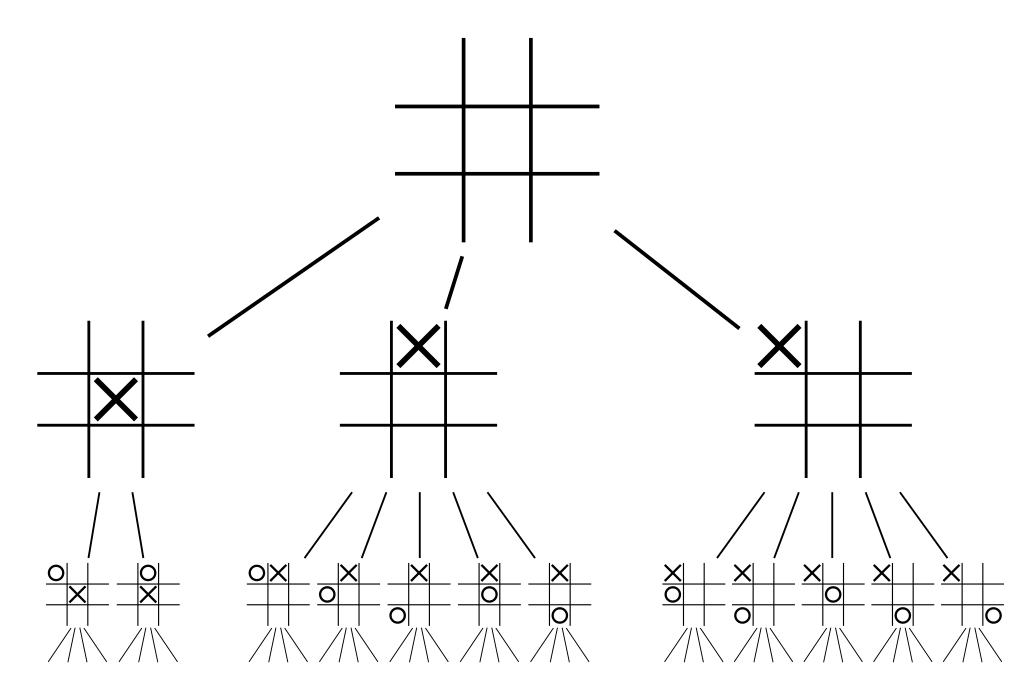
\includegraphics[width=0.7\linewidth]{1024px-Tic-tac-toe-game-tree}
	\caption[Ein Spielbaum mit den ersten zwei Zügen für Tic-Tac-Toe]{Ein Spielbaum mit den ersten zwei Zügen für Tic-Tac-Toe\protect\footnotemark}
	\label{fig:spielbaum}
\end{figure}

Spielbäume sind rekursive Datenstrukturen. Wenn ein Zug gewählt wurde, kann der verbleibende Teilbaum, mit dem gewählten Folgezustand nun in der Wurzel, als neuer Spielbaum wiederverwendet werden.

Ein einfacher Algorithmus, der aber bei großen Spielbäumen aber schnell an seine Grenzen stößt, um den optimalen Spielzug in einem Spielbaum zu wählen ist der \textbf{Minimax-Algorithmus}. 

\label{chap:minimax}
In einem Zwei-Spieler-Nullsummenspiel sind die Ziele beider Spieler exakt entgegengesetzt. Der eine Spieler versucht seinen (minimalen) Gewinn zu maximieren, während der Gegenspieler versucht, den (maximalen) Gewinn des ersten Spielers zu minimieren - daher der Name Minimax. Dies spiegelt sich auch im Minimax-Spielbaum wieder indem es Max-Knoten und Min-Knoten gibt. Bei Minimax wechseln sich die Knoten strikt ab, also Max-Knoten haben nur Min-Knoten als Kinder und umgekehrt. 

\footnotetext{\cite{en:user:gdrFirstTwoPly2007}}

\medskip
\begin{figure}[hbt!]
	\centering
	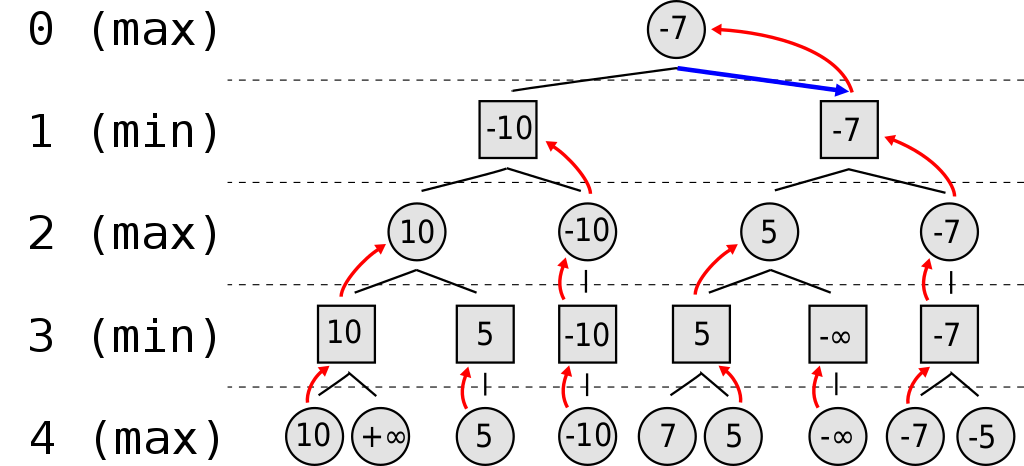
\includegraphics[width=0.7\linewidth]{1024px-Minimax}
	\caption[Minimax-Spielbaum]{Ein Minimax-Spielbaum mit Kreisen für Max-Knoten und Quadraten für Min-Knoten. Die roten Pfeile sind die gewählten Züge in jedem Knoten und der blaue Pfeil ist der gewählte Zug im Wurzelknoten. Die Zahlen in den Knoten stellen den Wert der Knoten dar. \protect\footnotemark }
	\label{fig:minimax}
\end{figure}
\footnotetext{\cite{nogueiraMinimaxAlgorithm2006}}

Minimax muss den gesamten Spielbaum erforschen, bis im Wurzelknoten ein optimaler Zug gewählt werden kann, da jeder Knoten von der Bewertung seiner Kindknoten abhängig ist. Bei Spielen mit großem Verzweigungsfaktor wie Schach und Go führt dies aber zu gigantischen Spielbäumen, die einfach nicht komplett aufgebaut werden können.

Eine Lösung für dieses Problem ist es einfach die Suche ab einer gewissen Tiefe zu beenden und den aktuellen Zustand mit einer Bewertungsfunktion zu bewerten. Dies hat sich aber zum Beispiel für Go als sehr schwierig herausgestellt, da es schwer ist eine angemessene Bewertungsfunktion zu definieren.

Die Alpha-Beta-Suche ist eine Modifikation der Minimax-Baumsuche, welche versucht nur so viel vom Spielbaum zu durchsuchen, wie es nötig ist. Sobald festgestellt wird, dass ein weiteres Kind in einem Knoten das Ergebnis nicht verbessern kann, wird der gesamte Teilbaum "abgeschnitten" und nicht weiter berücksichtigt.


\subsection{Der MCTS-Algorithmus}
\label{chap:mcts-algo}
Coulom kombinierte erstmals die Erzeugung eines Spielbaumes mit Monte-Carlo Simulationen. Unter Monte-Carlo Simulationen oder Monte-Carlo Experimenten versteht man gleichförmige Zufallsexperimente, die in großer Anzahl durchgeführt werden, um ein Ergebnis zu erhalten welches sich, mit steigender Anzahl der Experimente, dem tatsächlichen Wert immer weiter annähert.

Der von Coulom vorgestellt Algorithmus beginnt mit einem Knoten als Wurzel. Ausgehend von diesem Wurzelknoten werden nun zufällige Simulationen des Spiels gespielt. Das bedeutet in jedem Zustand wird ein zufälliger Zug gewählt und gespielt, bis das Spiel zu Ende ist. Der erste Zustand in einer solchen Simulation, der sich noch nicht im Spielbaum befindet, wird zum Baum hinzugefügt. Alle anderen Knoten, die sich bereits im Spielbaum befinden, merken sich, wie häufig sie bei solchen Simulationen besucht wurden und auch die Summe der Ergebnisse von Simulationen durch diesen Knoten. Die gesammelten Statistiken werden dann bei nachfolgenden Simulationen benutzt, um vielversprechende Knoten häufiger zu besuchen.

\begin{figure}[hbt!]
	\centering
	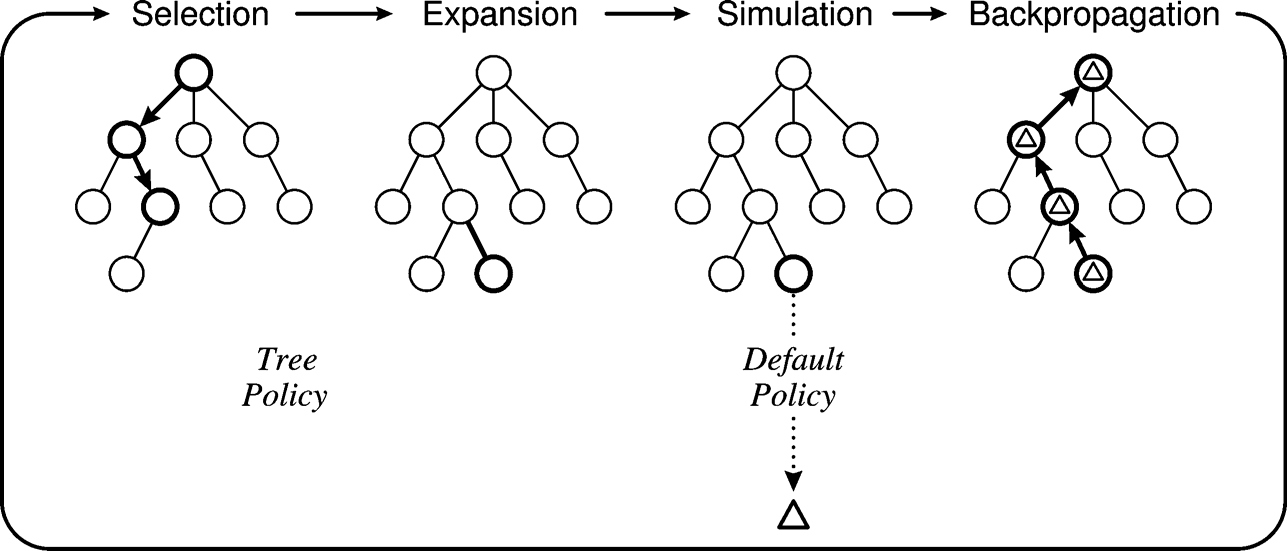
\includegraphics[width=0.7\linewidth]{mcts_survey_algorithm}
	\caption[Eine Iteration des MCTS Algorithmus]{Eine Iteration des MCTS Algorithmus\footnotemark}
	\label{fig:mctssurveyalgorithm}
\end{figure}
\footnotetext{\cite[\ppno~6]{browneSurveyMonteCarlo2012}}

Eine Iteration der Monte-Carlo-Baumsuche läuft in vier Schritten ab (siehe Abb. \ref{fig:mctssurveyalgorithm}). Zunächst wird der bestehende Spielbaum in einer \textbf{Selektions-Phase} durchlaufen, bis ein Blattknoten gefunden wurde. Dabei folgt der Algorithmus eine bestimmten Strategie (engl. policy) um die Knoten im Baum zu wählen. Ein Knoten ist ein Blatt des Baumes, wenn er terminal ist, oder noch nicht vollständig erforscht wurde, es also noch potentielle Kindknoten gibt, die noch nicht von diesem Knoten besucht wurden. Wenn dieser Blattknoten nicht terminal ist, so wird er \textbf{expandiert} indem ein noch nicht besuchtes Kind hinzugefügt und besucht wird. Ausgehend von diesem neuen Kindknoten wird nun eine \textbf{Simulation} gestartet. Es werden so lange zufällige Spielzüge ausgewählt bis das Spiel einen Endzustand erreicht hat. Die Strategie, die während der Simulation befolgt wird, nennt man auch die Default Policy. In der Regel werden die Spielzüge zufällig gewählt, es können aber Heuristiken benutzt werden um die Simulation zu steuern. Die Bewertung wird durch die Umgebung definiert, mit der der Algorithmus interagiert. Dafür benötigt die MCTS eine sogenannte Forward-Simulation der Umgebung. Die Umgebung muss aus einem Zustand $s$ und einer Aktion $a$ einen Folgezustand $s^\prime$ und eine Belohnung $r$ erzeugen können. Das Ergebnis dieser Simulation wird dann in der \textbf{Backup-Phase} benutzt, um die Bewertungen der in der Selektion besuchten Knoten zu aktualisieren. Die Problemstellung bestimmt, ob es nur terminale Belohnungen gibt, also nur wenn die Simulation einen Endzustand erreicht hat, oder ob jeder einzelne Zustandsübergang eine Belohnung liefert.

Diese vier Schritte werden so lange wiederholt, bis ein Ressourcenlimit, zum Beispiel ein Zeitlimit, erreicht ist. Danach wird der beste Zug im Wurzelknoten ausgewählt. Die Expansion und Selektion lassen sich logisch noch zu einer Einheit als Tree Policy zusammenfassen.
Der Ablauf ist in Algorithmus \ref{algo:mcts} als Pseudocode erklärt. Das Programm geht von einem Spielzustand $s_0$ im Wurzelknoten $v_0$ aus. $\textsc{TreePolicy}$ folgt einer festen Strategie, um ein Blatt $v_l$ im Baum zu finden, welches dann expandiert wird, wenn es möglich ist. $\textsc{SimuliereSpiel}$ arbeitet mit dem Spielzustand im Blatt $s(v_l) = s_l$ und erzeugt daraus eine Bewertung $r$. Diese Bewertung wird durch $\textsc{Backup}$ vom Blatt bis zur Wurzel propagiert und aktualisiert die Statistiken in den Knoten. Nach Ablauf eines Zeitlimits wird mit $\textsc{BestesKind}$ der am besten bewertete Kindknoten im Wurzelknoten $v_0$ gewählt und die zugehörige Aktion $a(v)$ zurückgegeben.

\begin{algorithm}[H]
\begin{algorithmic}
\Function{MCTS}{$s_0$}
	\State $v_0\gets$ Knoten($s_0$)
	\While{noch Zeit übrig}
		\State $v_l\gets \Call{TreePolicy}{v_0}$
		\State $r\gets \Call{SimuliereSpiel}{s(v_l)}$
		\State $\Call{Backup}{v_l, r}$
	\EndWhile

\State \textbf{return} $a(\Call{BestesKind}{v_0})$
\EndFunction
\end{algorithmic}
\caption{Allgemeiner MCTS Algorithmus\footnotemark}
\label{algo:mcts}
\end{algorithm}
\footnotetext{\cite[\ppno~5]{browneSurveyMonteCarlo2012}}

\subsection{Upper Confidence Bounds applied to Trees (UCT)}

Parallel zur Arbeit von Coulom haben Kocsis und Szepesv\'{a}ri 2006 den \textbf{Upper Confidence Bounds applied to trees} (UCT)-Algorithmus \autocite{kocsisBanditBasedMonteCarlo2006} entwickelt. UCT gilt heute als beliebtester MCTS-Algorithmus. Die Besonderheit von UCT liegt in seiner Tree Policy und damit in der Art, wie die Knoten im Baum ausgewählt werden. Kocsis und Szepesv\'{a}ri betrachten dabei die Auswahl eines Kindknotens als ein sogenanntes Banditenproblem. \autocite[\ppno~25\psqq]{suttonReinforcementLearningIntroduction2018}

\bigskip
Banditenprobleme sind eine Klasse von Problemen im bestärkenden Lernen, in denen der Agent zu jedem Zeitschritt $t$ aus $K$ Optionen wählen muss, um eine kumulative Belohnung zu maximieren, indem die optimale Aktion so oft wie möglich gewählt wird. Die Verteilung der Belohnungen jeder Aktion ist unbekannt aber statisch und die Belohnungen aus sukzessiven Aktionen sind voneinander unabhängig. Der Agent muss lernen, nur durch gesammelte Erfahrung seine erhaltene Belohnung auf lange Sicht zu maximieren. Verhält er sich gierig und wählt nur die Aktion mit der höchsten durchschnittlichen Belohnung, so werden alle Aktionen ignoriert, die im ersten Versuch keine Belohnung geliefert haben. Verbringt er dagegen zu viel Zeit damit, andere Aktionen als die derzeit beste zu erforschen, wählt er häufig suboptimale Aktionen. 

Dieses Problem, auch bekannt als \textbf{exploration-exploitation-Dilemma}, ist ein Grundproblem vieler Algorithmen des bestärkenden Lernens. Die beste Strategie für das Banditenproblem ist die upper confidence bound (UCB) Regel \textbf{UCB1} von Auer et.al \autocite[\ppno~237]{auerFinitetimeAnalysisMultiarmed2002}. Der Agent wählt die Aktion $j, 1 \le j \le K$, die die Gleichung

\begin{equation}
\bar{X}_j + \sqrt{\frac{2\ln n}{n_j}}
\label{eqn:UCB1}
\end{equation}

maximiert. Wobei $\bar{X}_j$ die durchschnittliche Belohnung ist, die bisher durch das Spielen von Aktion $j$ erhalten wurde, $n_j$ ist die Anzahl der Spielzüge in denen $j$ gewählt wurde und $n$ ist die Anzahl der insgesamt gespielten Spielzüge. Diese Gleichung besteht aus einem exploitation-Teil $\bar{X}_j$ und einem exploration-Teil $\sqrt{\frac{2\ln n}{n_j}}$. Der exploration-Teil repräsentiert die Unsicherheit in der Bewertung der Aktion $j$. Wenn die Aktion noch nicht oft gewählt wurde, $n_j$ also im Vergleich zu $n$ gering ist, so wird dieser Teil größer. Die Bewertung $\bar{X}_j$ ist noch sehr unsicher. Wurde dagegen $j$ sehr häufig gewählt, so wird der exploration-Teil kleiner und somit drücken wir eine hohe Sicherheit in der Schätzung des Wertes $\bar{X}_j$ aus.

\bigskip
Im UCT-Algorithmus wird die Auswahl des Kindknotens zu einem Banditenproblem. Dafür hat jeder Knoten $v$ eine Statistik $Q(v)$ mit der insgesamt erhaltene Belohnung in diesem Knoten und $N(v)$ mit der Anzahl der Besuche des Knotens. Das gewählte Kind ist dann jenes, welches die Formel

\begin{equation}
UCT = \frac{Q(v^\prime)}{N(v^ \prime)} + C_p\sqrt{\frac{\ln N(v)}{N(v^\prime)}}
\label{eqn:UCT}
\end{equation}

maximiert. Der Faktor $\sqrt{2}$ wurde aus der ursprünglichen UCB1-Formel (\ref{eqn:UCB1}) herausgezogen und als Parameter $C_p$ variierbar gemacht. Er kann für jedes Problem optimiert werden und bestimme Verbesserungen funktionieren besser mit verschiedenen Werten von $C_p$. Algorithmus \ref{algo:UCT} zeigt den vollen Pseudocode des UCT Algorithmus.

\begin{algorithm}[H]
\begin{algorithmic}[1]
\Function{UCT}{$s_0$}
	\State $v_0\gets$ Knoten($s_0$)
	\While{noch Zeit übrig}
		\State $v_l\gets$ \Call{TreePolicy}{$v_0$}
		\State $r\gets$ \Call{SimuliereSpiel}{$s(v_l)$}
		\State \Call{Backup}{$v_l, r$}
	\EndWhile 
	
\State \textbf{return} $a(\Call{BestesKind}{v_0,0})$
\EndFunction

\Function{TreePolicy}{$v$}
	\While{$v$ ist nicht terminal}
		\If{$v$ ist nicht vollständig expandiert}
			\State \textbf{return} \Call{Expandiere}{$v$}
		\Else
			\State $v \gets \textsc{BestesKind}(v)$
		\EndIf
	\EndWhile
	 
	\State \textbf{return} $v$
\EndFunction

\Function{Expandiere}{$v$}
	\State wähle $a \in$ noch nicht gewählte Aktionen aus $A(s(v))$
	\State füge ein neues Kind $v^\prime$ zu $v$ hinzu
	\State mit $s(v^\prime) = \textsc{Transition}(s(v),a)$
		\State und $a(v^\prime) = a$
		\State \textbf{return} $v^\prime$
\EndFunction

\Function{BestesKind}{$v, C_p$}\\
\State \textbf{return} $\argmax_{v^\prime \in\ \text{Kinder von}\ v} \frac{Q(v^\prime)}{N(v^\prime)} + C_p \sqrt{\frac{\ln N(v)}{N(v^\prime)}}$
\EndFunction

\Function{SimuliereSpiel}{$s$}
\While{$s$ ist nicht terminal}
\State wähle $a \in A(s)$ zufällig
\State $s \gets \textsc{Transition}(s,a)$
\EndWhile

\State \textbf{return} Belohnung für $s$
\EndFunction
\end{algorithmic}
\caption{Upper Confidence Bound applied to Trees\footnotemark}
\label{algo:UCT}
\end{algorithm}
\footnotetext{\cite[\ppno~7\psq]{browneSurveyMonteCarlo2012}}

Zusätzlich zu $Q(v)$ und $N(v)$ enthalten die Knoten noch Informationen über ihren Spielzustand $s(v)$ und die Aktion die in den Knoten geführt hat $a(v)$ sowie ein Verweis auf den Elternknoten. Die Backup-Regel ist unterschiedlich definiert für Ein-Spieler-Spiele und für Zwei-Spieler-Nullsummenspiele. Für Zwei-Spieler-Spiele in denen die Belohnungen für Spieler 1 gegenteilig zu den Belohnungen für Spieler 2 sind - $+1$ für Spieler 1 bedeutet $-1$ für Spieler 2 - kann die Belohnung des anderen Spielers durch Negierung in jedem Backup-Schritt erhalten werden.


\begin{algorithm}[H]
\begin{algorithmic}		
\Function{Backup}{$v, r$} \Comment{Ein-Spieler Backup}
	\While{$v$ ist nicht null}
		\State $N(v) \gets N(v) + 1$
		\State $Q(v) \gets Q(v) + r$
		\State $v \gets \text{Elternknoten von}\ v$
	\EndWhile
\EndFunction\\

\Function{Backup}{$v, r$} \Comment{Minimax Backup}
	\While{$v$ ist nicht null}
		\State $N(v) \gets N(v) + 1$
		\State $Q(v) \gets Q(v) + r$
		\State $r \gets -r$
		\State $v \gets \text{Elternknoten von}\ v$
	\EndWhile
\EndFunction
\end{algorithmic}
\caption{Backup-Regeln für Ein-Spieler und Zwei-Spieler Minimax}
\end{algorithm}

Dieser normale UCT (engl. plain UCT) Algorithmus, wie er von Kocsis und Szepesv\'{a}ri vorgestellt wurde, wird in Kapitel \ref{chap:mcts-impl} implementiert und als Ausgangslage für alle weiteren Verbesserungen genommen. 

\subsection{Verbesserungen}

Die verschiedenen Schritte der Baumsuche können verändert und verbessert werden und werden dadurch besser für die jeweiligen Anwendungsfälle geeignet. Im Paper "A survey of monte carlo methods" von Browne u.a.\autocite{browneSurveyMonteCarlo2012} wird eine große Menge von Verbesserungen vorgestellt und eine Übersicht darüber gegeben, für welche klassischen Spiele sie nützlich sein könnten. Im folgenden werde ich eine Handvoll ausgewählter Verbesserungen vorstellen.

\subsubsection{Transpositionen}
\label{transpos}
Unter Transpositionen versteht man identische Spielzustände, die über unterschiedliche Zugkombinationen erreicht werden. Ein solcher Spielzustand wird zum Beispiel über die Zugfolge d1,e1;c1,d2 erreicht (Abb. \ref{fig:c4transpos}).

\begin{figure}[hbt!]
	\centering
	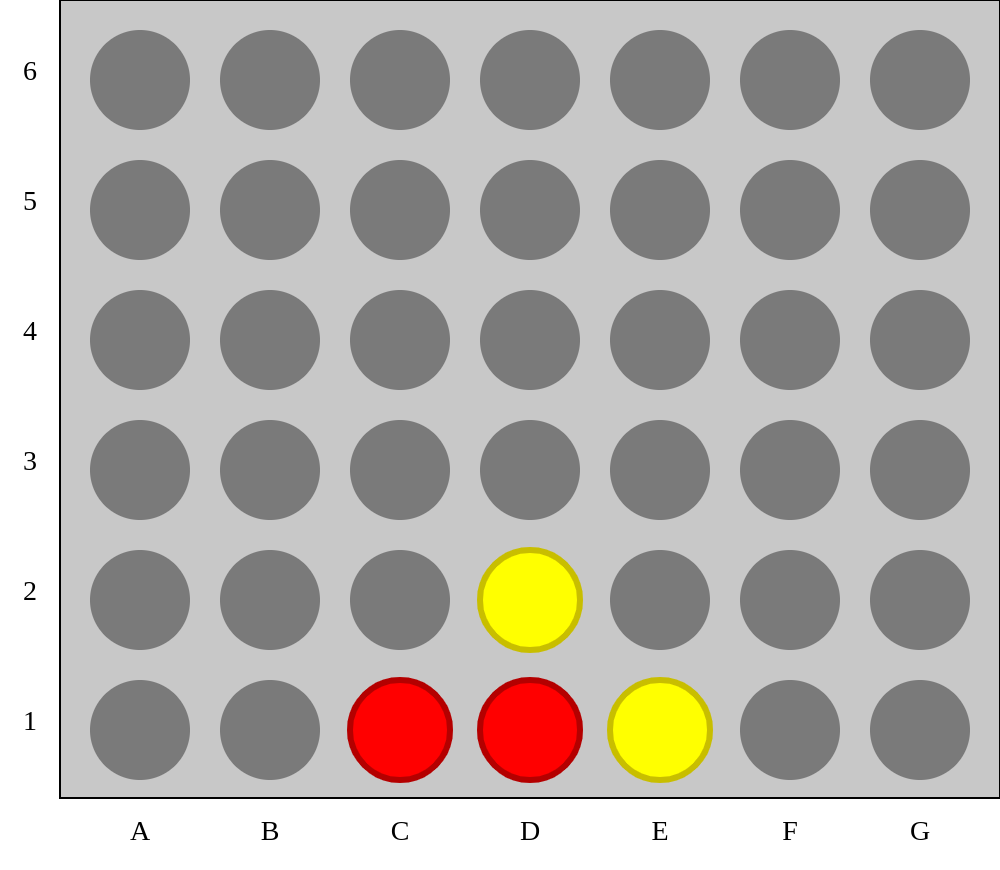
\includegraphics[width=0.7\linewidth]{c4_transpos}
	\caption[Transposition in Vier Gewinnt]{Die Spielposition kann auf mehrere Wegen erreicht werden. Die Züge d1,e1;c1,d2 sowie d1,d2;c1,e1 und c1,e1;d1,d2 führen alle zum selben Ergebnis.}
	\label{fig:c4transpos}
\end{figure}

Eine andere Zugfolge, die zum selben Spielzustand führt, ist d1,d2;c1,e1. Durch diese unterschiedlichen Pfade werden die beiden identischen Zustände normalerweise als separate Knoten mit separaten Statistiken gespeichert. Es würde aber sehr viel Sinn ergeben, diese Knoten zu kombinieren, denn der Weg, wie ein Zustand erreicht wird, hat keinen Einfluss darauf, welches die beste Aktion in diesem Zustand ist. Childs u.a. schlagen in ihrem Paper "Transpositions and Move Groups in Monte Carlo Tree Search"\autocite[\ppno~390\psq]{childsTranspositionsMoveGroups2008} drei Anpassungen des UCT-Algorithmus vor, um mit Transpositionen umzugehen. 

Normale UCT-Algorithmen, die Transpositionen nicht berücksichtigen, werden im Paper als \textbf{UCT0} bezeichnet. 

In Gleichung \ref{eqn:UCT} verwende ich die Statistiken eines Knotens $Q(v)$ und $N(v)$ direkt, also die Summe der Belohnungen aus Simulationen und die Anzahl an Simulationen durch diesen Knoten. Zusätzlich dazu kann diese Statistik abhängig von der gewählten Aktion $a$ im Knoten $v$, $Q(v,a)$ und $N(v,a)$ gespeichert werden. Wenn keine Transpositionen identifiziert werden, so sind die Werte identisch $v^\prime = \textsc{Transition}(s(v),a) \Rightarrow Q(v^\prime) = Q(v,a)$. Werden Transpositionen aber erkannt, kann es mehrere Aktionen in verschiedenen Knoten geben, die zum selben Kindknoten führen.

Wenn Transpositionen erkannt werden, so können sich im einfachsten Fall die Knoten, unabhängig davon wo sie sich im Baum befinden, ihre Statistiken teilen. Dies hat vor allem den Vorteil, dass der gesamte Baum kleiner wird. Die von Childs u.a. vorgeschlagene einfache Auswahlregel UCT1 ist:

\begin{equation}
UCT1 = \argmax_{a \in A(v)} \frac{Q(v,a)}{N(v,a)} + C_p\sqrt{\frac{\ln N(v)}{N(v,a)}}
\label{eqn:UCT1}
\end{equation}

Diese unterscheidet zwischen den verschiedenen Wegen, die zum selben Knoten geführt haben können, kumuliert aber die Statistiken von Knoten mit identischen Zuständen. Die zweite Vorgeschlagene Auswahlregel macht Gebrauch von mehr Informationen aus den Transpositionen, indem statt der Bewertung der Aktion $Q(v,a)$ die Bewertung des Folgezustands $Q(v^\prime)$ wie in der originalen UCT Implementierung verwendet wird (siehe Gleichung\~\ref{eqn:uct2}). Für die Berechnung des Erkundungsfaktors wird weiterhin $N(v,a)$ anstatt $N(v^\prime)$ im Nenner benutzt, da laut Childs die Auswahl sonst nicht mehr auf den korrekten Knoten konvergiert, wenn der der Knoten $v^\prime$ sehr häufig über einen anderen Pfad besucht wurde.

\begin{equation}
UCT2 = \argmax_{a \in A(v)} \frac{Q(v^\prime)}{N(v^\prime)} + C_p\sqrt{\frac{\ln N(v)}{N(v,a)}}
\label{eqn:UCT2}
\end{equation}

Die letzte vorgeschlagene Variante berechnet den Wert der Kinder $Q(v^\prime)$ rekursiv als gewichteter Durschnitt aller Kinder dieses Kindknotens. Dadurch, dass rekursiv alle Kinder eines Knotens betrachtet werden müssen, ist der Rechenaufwand in der Methode \textsc{bestesKind} sehr hoch. Um ihn zu reduzieren, können die Durchschnittswerte in den Knoten zwischengespeichert werden und müssen sich nur ändern, wenn sich ein Kind verändert. Damit kann der Rechenaufwand aus der teuren Selektionsphase in die Backupphase verlagert werden.

%TODO: UCT3 Gleichung
\begin{equation}
UCT3 = \argmax_{a \in A(v)}
\label{eqn:uct3}
\end{equation}

Durch das Kombinieren der Knoten entsteht ein gerichteter azyklischer Graph. Es kann nützlich sein, zur Bewertung eines Knotens nicht nur die direkten Kinder und Eltern zu betrachten, sondern beliebig tief im Graph auf- und abzusteigen. Cazenave, Mehat und Saffidine schlagen einen parametrisierbaren UCT Algorithmus, den sie Upper confidence bound for rooted directed acyclic graphs (UCD) nennen, vor. Sie zeigen wie mit dieser Parametrisierung die UCT1-3 Algorithmen von Childs u.a. implementiert werden können. Cazenave u.a. argumentieren dafür, die Statistiken nicht in den Knoten sondern in den Kanten zu speichern, dies kann allerdings die Implementierung verkomplizieren und wird deshalb bei der Anwendung von Transpositionen eher selten umgesetzt.
Der UCD-Algorithmus besteht aus drei Komponenten.
%TODO: UCD Gleichungen und Quelle
\begin{equation}
Gleichung1
\label{eqn:ucd1}
\end{equation}
\begin{equation}
Gleichung2
\label{eqn:ucd2}
\end{equation}
\begin{equation}
Gleichung3
\label{eqn:ucd3}
\end{equation}


\subsubsection{Scorebounded MCTS}
%TODO: Referenz Alpha-Beta Cuts, Scorebounded Quelle
Score bounded MCTS ist konzeptionell ähnlich zu Alpha-Beta Cuts im Minimax-Suchalgorithmus. Jeder Knoten speichert eine optimistische $opt(v)$ und pessimistische Grenze $pess(v)$ für seine Kindknoten. Die Bewertung hängt davon ab, ob der Knoten ein Min- oder ein Max-Knoten (siehe Seite \ref{chap:minimax}) ist.
Für einen Max-Knoten werden die optimistischsten, also die maximalen, Werte der Kinder genommen. Das heißt $opti(v) = \max_{k \in\ \text{Kinder von}\ v}opti(k)$ und $pess(v) = \max_{k \in\ \text{Kinder von}\ v}pess(k)$.
Ein Min-Knoten dagegen nimmt die minimalen Werte der Kinder $opti(v) = \min_{k \in\ \text{Kinder von}\ v}opti(k)$ und $pess(v) = \min_{k \in\ \text{Kinder von}\ v}pess(k)$.
Wenn ein Knoten terminal ist, so gilt $pess(v) = opti(v) = \textsc{Utility}(s(v),P_{max})$, die Grenzen entsprechen also der tatsächlichen Bewertung des Zustands durch die Umgebung aus Sicht des Max-Spielers. Der Einfachheit halber sind die Grenzen auch in einem Minimax-Baum immer aus Sicht des Max-Spielers definiert, das heißt bei terminalen Bewertungen von $[-1, 0, 1]$ für Niederlage, Unentschieden und Sieg ist ein Knoten mit $pess(v) = opti(v) = 1$ immer gut für den Max-Spieler respektive $pess(v) = opti(v) = -1$ ist immer schlecht für Max. Die Grenzen werden initialisiert mit $pess(v) = \textsc{Niederlage}, $opti(v) = \textsc{Sieg}$ und erst aktualisiert, wenn ein Endzustand \textbf{im Baum} erreicht wurde, also ein terminaler Blatt-Knoten dem Baum hinzugefügt wurde. Erst dann ist die tatsächliche Bewertung eines Knotens bekannt.

Die Grenzen können benutzt werden um Teile des Suchbaumes zu ignorieren, wenn durch die Grenzen bekannt ist, dass dieser Teilbaum die Bewertung nicht weiter verbessern kann, der Baum wird "beschnitten" (engl. pruned).
%TODO: Pruning genauer beschreiben.

Zusätzlich zum Beschneiden des Baumes können die Grenzen benutzt werden, um die Selektion zu beeinflussen. So können zum Beispiel Knoten mit einer hohen optimistischer Grenze bevorzugt besucht werden, während versucht wird Knoten mit geringer pessimistischer Grenze zu vermeiden. Zum Beispiel

\begin{equation}
Q_sb(v) = \frac{Q(v)}{N(v)} + \gamma opti(v) + \delta pess(v)
\label{eqn:scorebound}
\end{equation}

mit $-1 \le \gamma, \delta \le 1$.

Da die Grenzen eines Knotens von den Grenzen der Kindknoten abhängig ist, ist es notwendig die Grenzen so selten wie möglich zu aktualisieren und nicht bei jeder Iteration der Baumsuche neu zu berechnen. Dafür schlagen Cazenave und Saffidine zwei einfache Algorithmen vor, die die Grenzen aus einem terminalen Knoten effizient den gesamten Baum hinaufpropagieren.

%TODO: aktualisierungs-algorithmen abschreiben, quelle Scorebounded Seite X

\subsubsection{Rapid Action Value Estimation}

Rapid Action Value Estimation (RAVE) gehört zur Gruppe der All Moves as First (AMAF)-Verbesserungen. In der regulären Monte-Carlo-Baumsuche werden nur die tatsächlich besuchten Knoten in der Backup-Phase aktualisiert. Anstatt die besuchten Knoten und damit die konkreten Zustände zu betrachten, berücksichtigt die All Moves as First Verbesserung die gemachten Spiel\textbf{züge}. Der Gedanke dahinter ist, dass ein Spielzug $A$ der im Zustand $s_1$ gemacht wurde, in den Zuständen $s_t, t > 1$ genauso oder ähnlich gut ist. Im Schach ist zum Beispiel ein Zug, in dem ein Bauer eine stärkere Figur schlägt, (fast) immer gut, egal wie das restliche Spielfeld aussieht.

%TODO: Quelle für RAVE
Die verschiedenen AMAF-Verfahren unterscheiden sich dadurch, wie sie dieses Wissen speichern und verwenden. Manche verfahren aktualisieren die Statistik $Q(v)$ direkt, andere führen separate AMAF-Statistiken, um sie später gewichtet zu kombinieren. RAVE speichert die AMAF-Statistik $Q_RAVE(v)$ und $N_RAVE(v)$ separat und verwendet sie in der Selektionsphase bei der Auswahl der Kindknoten. Die Kombination der RAVE-Statistik mit der regulären MCTS-Statistik wird durch einen Parameter $\beta$ gesteuert.

\begin{equation}
UCT_{RAVE}=\beta * \frac{Q_RAVE(v^\prime)}{N_RAVE(v^\prime)} + (1-\beta) * \frac{Q(v^\prime)}{N(v^\prime)} + C_p * \sqrt{\frac{\ln(N(v))}{N(v^\prime)}
\label{eqn:uct-rave}
\end{equation}

\begin{equation}
\beta = \frac{N_{RAVE}(v^\prime)}{N(v^\prime)+N_{RAVE}(v^\prime)+N(v^\prime)*N_{RAVE}(v^\prime)*b^2}
\label{eqn:beta}
\end{equation}


Wenn dieser Parameter während der gesamten Baumsuche konstant bleibt, so nennt man diesen Algorithmus auch $\alpha$-AMAF, mit einem konstanten $\alpha \in [0,1]$. Das besondere an RAVE ist, dass sich dieser Parameter im Laufe der Baumsuche verändert. Wenn ein Knoten noch wenig besucht wurde, so ist $\beta$ nahe $1$, wodurch fast ausschließlich die RAVE-Statistik benutzt wird. Mit mehr Besuchen der Kindknoten, wird die gesammelte Statistik $Q(v)$ genauer und somit kann ein niedrigerer Wert für $\beta$ verwendet werden. Der Hyperparameter $b$ in Gleichung \ref{eqn:beta} kann angepasst werden, um RAVE gezielter anzupassn.

In der Selektions- und Simulations-Phase wird eine Liste aller gemachten Spielzüge geführt. Beim Backup werden dann auch alle Nachbarknoten im Baum aktualisiert, die durch einen der, später in der Simulation gemachten, Spielzüge erreicht werden könnten.

Was in der Literatur nicht erwähnt wird, ist die Notwendigkeit die Spielzüge eindeutig zu identifizieren. Die meisten Untersuchungen des Algorithmus beziehen sich nur auf Schach und Go, in denen ein Spielzug klar definiert ist (schwarzer Bauer von E2 nach E3 oder schwarzer Stein auf Kreuzung 3,3). Für Vier Gewinnt reicht es nicht, dass Spieler 1 einen Stein in Spalte 4 setzt, denn der tatsächlich resultierende Zug hängt davon ab, wie viele Steine sich bereits in der Spalte befinden. Darum muss jeder Zugname in Vier Gewinnt Informationen über den agierenden Spieler, die Spalte und die Zeile im Spielbrett enthalten.


\newpage
\section{Implementierung der Monte-Carlo-Baumsuche}
\label{chap:mcts-impl}

In diesem Kapitel werde ich meine Implementierungen der Monte-Carlo-Baumsuche und der ausgewählten Verbesserungen erklären.
Zunächst beschreibe ich kurz, wie das Spielfeld repräsentiert wird und wie die gemeinsame Schnittstelle der verschiedenen Agenten aussieht.
Danach stelle ich die Vergleichs-Algorithmen vor, die verwendet werden, um die korrekte Funktionsweise der Agenten sicherzustellen und um ihre optimalen Parameter zu bestimmen.
Anschließend wird zuerst die reine Monte-Carlo-Baumsuche ohne Verbesserung implementiert, dann wird sie um Transpositionserkennung erweitert.
Die Agenten für Scorebounded MCTS und RAVE MCTS sind ebenfalls Modifikationen der reinen Monte-Carlo-Baumsuche. Zum Schluss versuche ich die verschiedenen Verbesserungen zu kombinieren.

\subsection{Vier Gewinnt}
\label{chap:viergewinnt-impl}
Die Monte-Carlo-Baumsuche benötigt eine Simulation der Umgebung.
Der Kaggle-Wettbewerb liefert bereits mit dem Python Package \verb|kaggle-environments| eine Spielumgebung für ein parametrisierbares Vier Gewinnt.
Diese Umgebung wird vom Wettbewerb selbst für die Evaluierung der eingereichten Agenten verwendet, ist aber für meine Zwecke unnötig Umfangreich und unbequem zu verwenden.

Deshalb war es zuerst notwendig, eine eigene Implementierung von Vier Gewinnt zu erstellen.
Die Klasse \verb|bachelorarbeit.games.ConnectFour| ist eine Erweiterung der Logik aus dem \verb|connectx.py| Modul von kaggle-environments\footnote{Quelle: https://github.com/Kaggle/kaggle-environments/tree/master/kaggle_environments/envs/connectx}.

Das Spielfeld wird in einer Liste der Länge \verb|anzahl_spalten * anzahl_zeilen| gespeichert.
Ein leeres Feld wird durch eine 0, Steine von Spieler 1 und 2 durch die Zahlen 1 und respektive 2 repräsentiert.
Index 0 ist  die obere linke Zelle des Spielfeldes, der letzte Index ist die untere rechte Zelle.
Die oberste Zeile des Spielfeldes entspricht den ersten \verb|anzahl_spalten| Werten der Liste.

Diese Repräsentation lässt sich leicht in eine zwei-Dimensionale Darstellung umwandeln.

Die wichtigsten Methoden der Klasse \verb|ConnectFour| sind
\begin{itemize}
	\item \verb|play_move(column)| Setzt einen Stein für den aktuellen Spieler in die angegebene Spalte
	\item \verb|list_moves()| Listet alle legalen Spielzüge
	\item \verb|is_terminal()| Gibt \verb|True| zurück, wenn das Spiel vorbei ist, sonst \verb|False|
	\item \verb|get_reward(player)| Gibt die Belohnung für den angegebenen Spieler zurück.\\1 bei einem Sieg, -1 bei einer Niederlage und sonst 0.
\end{itemize}

Zusätzlich kann sich ein Objekt der Klasse selbst kopieren und kann einen Hash des Spielzustandes erzeugen.
Dieser Hash ist für die Transpositionstabelle nötig.

\subsection{Die Schnittstelle}
\label{chap:schnittstelle}
Jeder Agent erbt von der Klasse \verb|bachelorarbeit.base_players.Player|.
Diese Basisklasse gibt die Schnittstelle des Agenten vor.
Es ist notwendig, dass ein Agent die Methode \verb|get_move(Observation, Configuration) -> int| implementiert.

\verb|Observation| und \verb|Configuration| sind zwei Datenstrukturen der Kaggle Umgebung.
In diesem Projekt sind sie im Modul \verb|bachelorarbeit.games| als Python \verb|DataClass| umgesetzt.
Die \verb|Observation| ist der aktuelle Zustand der Spielumgebung.
Sie enthält das Spielfeld als \verb|Observation.board| im selben Format wie oben beschrieben und das Zeichen (\verb|1| oder \verb|2|) des Spielers der am Zug ist.
\verb|Configuration| enthält die Informationen über die Konfiguration des Spiels selbst.
Dies sind die Anzahl der Spalten \verb|Configuration.columns| und Zeilen \verb|Configuration.rows| des Spielfelds, die Anzahl der, für den Sieg nötigen, Steine in einer Reihe \verb|Configuration.inarow| und ein Zeitlimit für die Ausführung des Agenten.

Im Wettbewerb hat jeder Agent eine Vorbereitungszeit beim ersten Zug von 10 Sekunden und für jeden weiteren Zug 5 Sekunden.
Da allerdings die Leistung der Maschinen, auf denen der Wettbewerb ausgeführt wird, nur schwer eingeschätzt werden kann, benutze ich lokal kein Zeitlimit für meine Agenten.
Stattdessen wird die Baumsuche auf eine bestimmte Anzahl an Iterationen limitiert.

Der Rückgabewert der Methode ist der Zug, den der Agent macht, also eine Zahl zwischen 0 und \verb|anzahl_spalten-1|.

\begin{lstlisting}[language=Python,caption=Die Basisklasse aller Agenten.,label={lst:baseplayer}]
class Player(ABC):
    name = "Player"

    @abstractmethod
    def get_move(self, observation: Observation, configuration: Configuration) -> int:
        pass
\end{lstlisting}

\subsection{Vergleichsalgorithmen}
\label{chap:vergleiche-impl}

Die Agenten werden mit einer Reihe verschiedener Algorithmen verglichen.
Der einfachste Vergleich ist gegen einen rein zufälligen Spieler \verb|bachelorarbeit.base_players.RandomPlayer|.
Dieser Spieler wählt immer einen zufälligen legalen Zug.
Wenn es einem Agenten nicht gelingt nahezu einhundert Prozent der Spiele gegen den zufälligen Spieler zu gewinnen, so muss etwas an ihrer Implementierung fehlerhaft sein.

\begin{lstlisting}[language=Python,caption=Ein Spieler der zufällige Züge wählt.,label={lst:randomplayer}]
class RandomPlayer(Player):
    name = "RandomPlayer"

    def get_move(self, observation: Observation, configuration: Configuration) -> int:
        return random.choice([c for c in range(configuration.columns) if observation.board[c] == 0])
\end{lstlisting}

Der zweite Vergleich ist gegen einen Algorithmus der auch Flat Monte Carlo, also flache Monte Carlo Suche (Flat MC), genannt wird.
Flat Monte Carlo erzeugt nur einen minimalen Spielbaum.
Er besteht nur aus der Wurzel und ihren direkten Kindknoten.
In jedem Schritt wird eine Aktion gleichmäßig zufällig ausgewählt und das Spiel ab diesem Zustand zufällig zu Ende simuliert.
Das Ergebnis dieser Simulation wird für diese Aktion gespeichert.
Der Agent führt zufällige Iterationen durch, bis ein Zeit oder Schrittlimit erreicht ist.
Am Ende wird die Aktion gewählt, die die höchste durchschnittliche Bewertung hat.
Eine stärkere Variante dieses Spielers wählt die Kindknoten nicht zufällig sondern mit der UCB-Formel (Gleichung~\ref{eqn:ucb}) aus.

\begin{lstlisting}[language=Python,caption=Flache Monte Carlo Suche.,label={lst:flat-mc}]
class FlatMonteCarlo(Player):
    name = "FlatMonteCarloPlayer"

    def __init__(self, max_steps: int = 1000, exploration_constant: float = 1.0, ucb_selection: bool = True, **kwargs):
        super(FlatMonteCarlo, self).__init__(**kwargs)
        self.max_steps = max_steps
        self.ucb_selection = ucb_selection
        self.exploration_constant = exploration_constant

    def evaluate_game_state(self, game: ConnectFour, scoring_player: int) -> int:
        while not game.is_terminal():
            move = random.choice(game.list_moves())
            game.play_move(move)

        return game.get_reward(scoring_player)

    def get_move(self, observation: Observation, configuration: Configuration) -> int:
        game = ConnectFour(board=observation.board, rows=configuration.rows,
                           columns=configuration.columns, inarow=configuration.inarow,
                           mark=observation.mark)

        visits = defaultdict(int)  # Anzahl der Simulationen pro Aktion
        rewards = defaultdict(int)  # Summe der Bewertungen pro Aktion
        scoring_player = game.get_current_player()

        def move_score(move: int, steps_elapsed: int, exploration: float) -> float:
            if visits[move] == 0:
                return 10  # Erzwinge Selektion von unerforschten Zügen
            else:
                # UCB Auswahl-Regel
                return rewards[move] / visits[move] \
                       + exploration * math.sqrt(2 * math.log(steps_elapsed) / visits[move])

        for i in range(self.max_steps):
            if self.ucb_selection:
                move = max(game.list_moves(), key=lambda m: move_score(m, i + 1, self.exploration_constant))
            else:
                move = random.choice(game.list_moves())
            result = self.evaluate_game_state(game.copy().play_move(move), scoring_player)
            visits[move] += 1
            rewards[move] += result

        chosen_move = max(visits.keys(), key=lambda m: move_score(m, 1, 0))

        return chosen_move
\end{lstlisting}

Der Flat Monte Carlo Spieler kann durch den Parameter \verb|max_steps| und die Variante mit UCB-Kindauswahl zusätzlich mit dem Parameter \verb|exploration_constant| konfiguriert werden.
In den Vergleichen mit anderen Agenten sind die Parameter allerdings auf \verb|max_steps=1000, exploration_constant=1.0| fixiert.

Der Wert des \verb|exploration_constant| Parameters wurde experimentell bestimmt, indem der Agent gegen sich selbst gespielt hat.
Dafür wurde der Parameter für einen Spieler auf 1.0 fixiert, und mit verschiedenen Werten des anderen Spielers verglichen.
Die Ergebnisse sind in Tabelle~\ref{tab:flat-mc}.

\begin{table}[h!]
\centering
\begin{tabular}{ |c||c|c|c|c|c|c|c|c| }
 \hline
 $C_p$ & 0.1 & 0.25 & 0.5 & $\frac{1}{\sqrt{2}}$ & 1.0 & 1.2 & $\sqrt{2}$ & 2.0 \\
 \hline
 Gewinnchance & 0.05 & 0.22 & 0.455 & 0.48 & 0.495 & 0.445 & 0.515 & 0.455 \\
 \hline
\end{tabular}
\caption{Gewinnchance für unterschiedliche Werte des \verb|exploration_constant| Parameters über 300 Spiele. Die Hälfte der Spiele hat der Spieler angefangen, die andere hälfte hat er als zweites gezogen.}
\label{tab:flat-mc}
\end{table}

Die dritte Art der Evaluation geschieht mit einem Datensatz aus 1000 Spielpositionen und Bewertungen jedes Zuges in dieser Position durch einen perfekten Spieler.
Der Datensatz wurde vom Nutzer Peter Cnudde mit einem Vier Gewinnt Solver, einem in C++ geschriebenen Programm, das für jeden Zustand die optimalen Spielzüge berechnen kann, erstellt und auf Kaggle hochgeladen\footnote{Quelle: https://www.kaggle.com/petercnudde/scoring-connect-x-agents}.
Jede Spielposition in diesem Datensatz hat das folgende Format:

\begin{verbatim}
{"board": [0, 0, 0, 0, 0, 0, 0, 0, 0, 2, 0, 0, 0, 2, 0, 0, 2, 0, 0, 0, 1, 0, 0, 1, 0, 0, 0, 2, 1, 0, 2, 0, 0, 0, 1, 1, 1, 2, 1, 0, 1, 2], "score": -2, "move score": [-3, -4, -4, -2, -6, -5, -4]}
\end{verbatim}

\verb|board| ist der Zustand des Spielfeldes, \verb|score| ist die maximal erzielbare Bewertung und \verb|move score| enthält die Bewertungen aller Spielzüge aus diesem Zustand.
Eine Bewertung = 0 bedeutet das Spiel endet unentschieden, eine Bewertung > 0 bedeutet dass der Spieler gewinnt (je größer der Wert, desto schneller gewinnt der Spieler) und < 0 bedeutet der Spieler verliert.
Ist eine Bewertung = -99 so ist dieser Zug nicht legal.
Die Bewertung des Agenten basiert auf zwei Metriken:
\begin{itemize}
    \item Gute Züge: Zustände in denen eine Aktion gewählt wurde, die das selbe Spielergebnis zur Folge hat, wie der optimale Zug.\\Also beispielsweise ein Zug mit positiver Bewertung, falls der Spieler gewinnen könnte.
    \item Perfekte Züge: Zustände in denen die Aktion gewählt wurde, die den selben Wert hat, wie die optimale Bewertung durch den perfekten Spieler.
\end{itemize}

Da die, durch die Baumsuche gewählten, Spielzüge auch durch Zufall beeinflusst sind, wird die Evaluation für jeden Spieler und jede Konfiguration mehrfach durchgeführt.
Die Punktzahlen des zufälligen Spielers und des Flat Monte Carlo Spielers sind in Tabelle~\ref{tab:move-evaluation-baseline} gelistet.
Die MCTS-Agenten müssen diese Werte übertreffen.

\begin{table}[h!]
\centering
\begin{tabular}{ |c||c|c| }
 \hline
 Spieler & Gut & Perfekt //
 \hline
 Zufällig & 0.67 & 0.25 //
 \hline
 Flat MC & 0.75 & 0.55 //
\end{tabular}
\caption{Prozentsatz der guten und perfekten Züge im Datensatz mit 1000 Spielpositionen für den zufälligen und den Flat Monte Carlo Spieler. Jede Evaluation wurde 10 mal wiederholt und der Durchschnitt der Ergebnisse gebildet. Der Flat Monte Carlo Spieler benutzt die UCB-Formel zur Kindauswahl mit der Konstanten $C_p=1.0$ und hat 1000 Iterationen Bedenkzeit pro Zug.}
\label{tab:move-evaluation-baseline}
\end{table}

\subsection{Normale Monte-Carlo-Baumsuche}
\label{subsec:normale-monte-carlo-baumsuche}

Die Monte-Carlo-Baumsuche ist in zwei Klassen im Modul \verb|bachelorarbeit.mcts| implementiert.
Der Spielbaum besteht aus Knoten der Klasse \verb|Node|.
Jeder Knoten speichert die für den UCT-Algorithmus notwendigen Statistiken $Q(v)$ und $N(v)$ als \verb|average_value| und \verb|number_visits| sowie Verweise zu den Kindknoten und dem Elternknoten.
Die Methoden sind im Programm-Code kurz zusammengefasst.

\begin{lstlisting}[language=Python,caption=Der Knoten der Monte-Carlo-Baumsuche,label={lst:mcts-node}]
class Node:
    def __init__(self, game_state: ConnectFour, parent: Node = None):
        self.average_value = 0  # Q(v)
        self.number_visits = 0  # N(v)
        self.children = {}  # C(v), Kinder des Knotens

        self.parent = parent  # der direkte Elternknoten

        self.game_state = game_state  # der Spielzustand in diesem Knoten
        self.possible_moves = game_state.list_moves()  # Aktionen für die noch nicht erforschten Kindknoten
        self.expanded = False  # ob der Knoten vollständig expandiert ist

    def best_child(self, exploration_constant: float = 1.0) -> "Node":
        """Gibt das Kind mit dem höchsten UCT-Wert zurück"""
        n_p = math.log(self.number_visits)

        def UCT(child: Node):
            """
            Berechnet den UCT Wert UCT = Q(v') + C_p * sqrt(ln(N(v))/N(v'))
            :param child: Knoten v'
            :return:
            """
            return child.Q() + exploration_constant * math.sqrt(n_p / child.number_visits)

        _, c = max(self.children.items(), key=lambda entry: UCT(entry[1]))
        return c

    def increment_visit_and_add_reward(self, reward: float):
        """Aktualisiert die Statistik dieses Knotens"""
        self.number_visits += 1
        self.average_value += (reward - self.average_value) / self.number_visits

    def expand_one_child(self) -> "Node":
        """ Wählt einen zufälligen Spielzug aus und erzeugt den dazugehörigen Kindknoten"""

\end{lstlisting}

Der Spieler \verb|MCTSPlayer| implementiert den "Upper Confidence Bound for Trees"-Algorithmus aus Kapitel~\ref{algo:uct} direkt.
Die Methode \verb|get_move| enthält zusätzliche Logik um den Spielbaum von einem Spielzug zum nächsten beizubehalten.
Der eigentliche Algorithmus ist in der Methode \verb|perform_search(root: Node)| implementiert.

\begin{lstlisting}[language=Python,caption=Die MCTSPlayer Klasse,label={lst:mcts-player}]

class MCTSPlayer(Player):
    name = "MCTSPlayer"

    def __init__(self, exploration_constant: float = 1.0,
                 max_steps: int = 1000, keep_tree: bool = False, **kwargs):
        super(MCTSPlayer, self).__init__(**kwargs)

        self.exploration_constant = exploration_constant  # UCT Exploration Konstante Cp
        self.keep_tree = keep_tree  # behalte den Baum zwischen Zügen
        self.root = None  # die Wurzel des Baumes

    def get_move(self, observation: Observation, conf: Configuration) -> int:
        self.reset(conf)  # Da der Spieler zwischen Zügen persistent ist, können hier Variablen pro Zug zurückgesetzt werden

        # An dieser Stelle wird der aktuelle Zustand im Baum gesucht, falls der Baum zwischen Zügen erhalten bleibt
        root = self._restore_root(observation, conf)

        # Wenn keine Wurzel gefunden wurde, wird ein neuer Baum erstellt
        if root is None:
            root_game = ConnectFour(columns=conf.columns, rows=conf.rows, inarow=conf.inarow,
                                    mark=observation.mark, board=observation.board)
            root = self.init_root_node(root_game)

        # Führt die eigentliche Suche aus
        best = self.perform_search(root)

        # Speichert den Wurzelknoten für den nächsten Zug
        self._store_root(root.children[best])

        return best

    def perform_search(self, root) -> int:
        while self.has_resources():
            leaf = self.tree_policy(root)
            reward = self.evaluate_game_state(leaf.game_state)
            self.backup(leaf, reward)
        return self.best_move(root)

    def tree_policy(self, root: Node) -> Node:
        current = root
        while not current.game_state.is_terminal():
            if current.is_expanded():
                current = current.best_child(self.exploration_constant)
            else:
                return current.expand_one_child()
        return current

    def evaluate_game_state(self, game_state: ConnectFour) -> float:
        game = game_state.copy()
        # Die Bewertung Geschieht aus Sicht des Spielers, der uns in diesen Zustand geführt hat, darum muss der Spieler
        # geholt werden, der zuletzt gezogen hat, nicht der der gerade an der Reihe ist.
        scoring = game.get_other_player(game.get_current_player())
        while not game.is_terminal():
            game.play_move(random.choice(game.list_moves()))

        return game.get_reward(scoring)

    def backup(self, node: Node, reward: float):
        current = node
        while current is not None:
            current.increment_visit_and_add_reward(reward)
            reward = -reward
            current = current.parent

\end{lstlisting}

Die anpassbaren Parameter der verb|MCTSPlayer|-Klasse sind, die Anzahl der Iterationen pro Spielzug \verb|max_steps|, die Konstante \verb|exploration_constant| $C_p$ und das Beibehalten des Baumes zwischen Zügen.
Um eine vergleichbare Grundlage zu haben, werden alle MCTS-Varianten mit 1000 Iterationen pro Zug getestet und verglichen.
Manche Verbesserungen benötigen mehr Rechenzeit für 1000 Iterationen, weshalb ich in Kapitel~\ref{chap:results} auch noch Vergleiche bei gleicher Ausführungszeit durchführen werde.

Zunächst habe ich den Agent gegen den zufälligen Spieler antreten lassen.
Der Parameter \verb|exploration_constant| wurde, ausgehend vom Flat Monte Carlo Spieler, als Standardwert auf 1.0 gesetzt und der Baum wird nicht zwischen Spielzügen behalten.
Von 100 Spielen hat der Agent 100 Prozent gewonnen.

Als nächstes wurde der Agent mit dem Flat Monte Carlo Spieler mit UCB-Kindauswahl verglichen.
Wieder wurden Werte der \verb|exploration_constant| zwischen $0.1$ und $2.0$ getestet, um einen optimalen Wert zu bestimmen.
Die Ergebnisse der Parameter mit \verb|keep_tree=False| und \verb|keep_tree=True| sind in Tabelle~\ref{tab:mcts-flat-mc} zu finden.

\begin{table}[h!]
\centering
\begin{tabular}{ |c||c|c|c|c|c|c|c|c| }
 \hline
 $C_p$ & 0.1 & 0.25 & 0.5 & $\frac{1}{\sqrt{2}}$ & 1.0 & 1.2 & $\sqrt{2}$ & 2.0 \\
 \hline
 \verb|keep_tree=False| & 0.06 & 0.22 & 0.455 & 0.48 & 0.495 & 0.445 & 0.515 & 0.455 \\
 \hline
 \verb|keep_tree=True| & 0.06 & 0.22 & 0.455 & 0.48 & 0.495 & 0.445 & 0.515 & 0.455 \\
 \hline
\end{tabular}
\caption{Gewinnchance der MCTS gegen FlatMC über 300 Spiele für verschiedene Parameter.}
\label{tab:mcts-flat-mc}
\end{table}

Die Experimente Zeigen, dass eine \verb|exploration_constant| nahe 1.0 die besten Ergebnisse liefert und dass die Spielstärke ansteigt, wenn der Spielbaum zwischen Zügen erhalten bleibt.

In der Evaluation der Spielpositionen wird jeder Spielzug einzeln bewertet.
Dadurch gibt es keine vorherigen Spielzüge, aus denen der Spielbaum wiederverwendet werden kann.
Deshalb wird nur der Parameter $C_p$ mit Werten nahe 1.0 verglichen.

\begin{table}[h!]
\centering
\begin{tabular}{ |c||c|c| }
 \hline
 $C_p$ & Gut & Perfekt //
 \hline
 0.7 & 0.67 & 0.25 //
 \hline
 0.8 & 0.67 & 0.25 //
 \hline
 0.9 & 0.67 & 0.25 //
 \hline
 1.0 & 0.67 & 0.25 //
 \hline
 1.1 & 0.67 & 0.25 //
 \hline
 1.2 & 0.67 & 0.25 //
 \hline
\end{tabular}
\caption{Prozentsatz der guten und perfekten Züge im Datensatz mit 1000 Spielpositionen für die normale Monte-Carlo-Baumsuche. Jede Evaluation wurde 10 mal wiederholt und der Durchschnitt der Ergebnisse gebildet.}
\label{tab:move-evaluation-mcts}
\end{table}

Auch hier zeigt sich, dass ein Parameter $C_p$ nahe 1.0 die besten Ergebnisse liefert.
Der optimierte MCTS-Agent wird für die Verbesserungen als Vergleich benutzt.
Im direkten Vergleich muss eine Verbesserung mehr als 50\% der Spiele gegen den normalen MCTS-Agent gewinnen um als besser zu gelten.

\subsection{MCTS mit Transpositionen}
\label{subsec:mcts-mit-transpositionen}

Bei der Implementierung der Transpositionen habe ich mich dafür entschieden, die UCT1 und UCT2 Algorithmen \refpage{eqn:uct1} von Childs u.a.\ zu implementieren.
Dafür war es notwendig, dass die Knoten zusätzlich zu ihren eigenen Statistiken $Q(v)$ und $N(v)$ auch die Informationen über die, von ihnen erreichten, Kindknoten $Q(v,a)$ und $N(v,a)$ speichern.
Diese zusätzlichen Statistiken werden in der Methode \verb|best_child| verwendet, um UCT1 bzw.\ UCT2 zu implementieren.

\begin{lstlisting}[language=Python,label={lst:transpos-node}]
from bachelorarbeit.mcts import Node
from collections import defaultdict
import math
import random

class TranspositionNode(Node):
    def __init__(self, *args, **kwargs):
        super(TranspositionNode, self).__init__( *args, **kwargs)
        self.child_values = defaultdict(float)
        self.child_visits = defaultdict(int)

    def Qsa(self, move):
        return self.child_values[move]

    def Nsa(self, move):
        return self.child_visits[move]

    def best_child(self, exploration_constant: float = 1.0, uct_method: str = "UCT") -> "Node":
        n_p = math.log(self.number_visits)

        parent = self

        def UCT1(action, _):
            return parent.Qsa(action) + exploration_constant * math.sqrt(n_p / parent.Nsa(action))

        def UCT2(action, child):
            return child.Q() + exploration_constant * math.sqrt(n_p / parent.Nsa(action))

        def default(_, child):
            return child.Q() + exploration_constant * math.sqrt(n_p / child.number_visits)

        selection_method = default
        if uct_method == "UCT1":
            selection_method = UCT1
        elif uct_method == "UCT2":
            selection_method = UCT2

        _, c = max(self.children.items(), key=lambda ch: selection_method(*ch))
        return c

    def get_random_action_and_state(self) -> Tuple[int, ConnectFour]:
        m = random.choice(self.possible_moves)
        self.possible_moves.remove(m)
        if len(self.possible_moves) == 0:
            self.expanded = True

        s = self.game_state.copy().play_move(m)
        return m, s
\end{lstlisting}

Die \verb|MCTSPlayer|-Klasse wurde um ein \verb|dict| Erweitert, das die Transpositionen speichert.
Der Schlüssel dieses Dicts ist der Hash des Spielzustandes und der Wert ist der dazugehörige Knoten.
Wenn in der Expansionsphase in \verb|tree_policy()| ein neuer Knoten erzeugt würde, so wird zunächst der Hash des korrespondierenden Spielzustandes erzeugt, und geprüft ob sich dieser Hash bereits in der Transpositionstabelle befindet.
Wenn er bereits vorhanden ist, so wird der gespeicherte Knoten wiederverwendet und als neues Kind des expandierenden Knotens benutzt.
Ist der Zustand noch nicht in der Transpositionstabelle, so wird ein komplett neuer Knoten erzeugt und im Dict gespeichert.
Da die Baumsuche auf eine maximale Anzahl an Iterationen begrenzt wird, sollte es keine Probleme mit der Größe der Transpositionstabelle geben.
Bei lange laufenden Algorithmen kann es aber nötig sein, alte Knoten aus der Tabelle zu entfernen, um den Speicherverbrauch zu limitieren.

Da der Baum durch die Transpositionen zu einem gerichteten Graph wird, kann jeder Knoten mehrere Elternknoten haben.
Dadurch kann die Belohnung in \verb|backup| nicht mehr über den Elternknoten bis zur Wurzel propagiert werden, da der korrekte Pfad daraus nicht ersichtlich ist.
Um dieses Problem zu lösen, wird in \verb|tree_policy| eine Liste der Knoten, die in der Selektionsphase besucht wurden, erzeugt und diese Liste wird in \verb|backup| rückwärts durchlaufen.
In \verb|backup| werden zusätzlich noch die Kind-Statistiken $Q(v,a)$ und $N(v,a)$ der jeweiligen Elternknoten aktualisiert.

\begin{lstlisting}[language=Python,label={lst:transposition-player}]
class TranspositionPlayer(MCTSPlayer):
    name = "Transpositionplayer"

    def __init__(self, uct_method: str = "UCT", **kwargs):
        super(TranspositionPlayer, self).__init__(**kwargs)
        self.transpositions = {}
        self.uct_method = uct_method

    def tree_policy(self, root: TranspositionNode) -> List[TranspositionNode]:
        current = root
        path = [root]  # Der Pfad, der während der Selektion durchlaufen wird
        while not current.game_state.is_terminal():
            if current.is_expanded():
                current = current.best_child(self.exploration_constant, uct_method=self.uct_method)
                path.append(current)
            else:
                # Wähle einen zufälligen nächsten Zustand
                move, next_state = current.get_random_action_and_state()
                # Und prüfe ob er bereits in der Transpositionstabelle enthalten ist
                hash_state = hash(next_state)
                if hash_state not in self.transpositions:
                    # Wenn nicht wird ein neuer Knoten hinzugefügt
                    self.transpositions[hash_state] = TranspositionNode(game_state=next_state, parent=current)
                next_node = self.transpositions[hash_state]
                current.add_child(next_node, move)
                path.append(next_node)
                return path
        return path

    def backup(self, path: List[TranspositionNode], reward: float):
        prev = None
        for _node in reversed(path):
            _node.increment_visit_and_add_reward(reward)

            if prev is not None:
                m = _node.find_child_action(prev)
                _node.increment_child_visit_and_add_reward(m, -reward)

            prev = _node
            reward = -reward
\end{lstlisting}

Für beide Selektionsverfahren UCT1 und UCT2 wird separat der optimale Parameter $C_p$ bestimmt indem der Agent gegen den Flat Monte Carlo Spieler spielt.

\begin{table}[h!]
\centering
\begin{tabular}{ |c||c|c|c|c|c|c|c|c| }
 \hline
 $C_p$ & 0.1 & 0.25 & 0.5 & $\frac{1}{\sqrt{2}}$ & 1.0 & 1.2 & $\sqrt{2}$ & 2.0 \\
 \hline
 \verb|UCT1| & 0.06 & 0.22 & 0.455 & 0.48 & 0.495 & 0.445 & 0.515 & 0.455 \\
 \hline
 \verb|UCT2| & 0.06 & 0.22 & 0.455 & 0.48 & 0.495 & 0.445 & 0.515 & 0.455 \\
 \hline
\end{tabular}
\caption{Gewinnchance von MCTS mit Transpositionen gegen FlatMC über 300 Spiele für verschiedene Parameter $C_p$.}
\label{tab:transpos-flat-mc}
\end{table}

Auch mit Transpositionen scheint die Konstante $C_p$ einen optimalen Wert nahe 1.0 zu haben.
Die Zug-Evaluation bestätigt diese Vermutung.

\begin{table}[h!]
\centering
\begin{tabular}{ |c|c||c|c|c|c|c|c|c|c| }
 \hline
 \multicolumn{2}{|c|}{$C_p$} & 0.1 & 0.25 & 0.5 & $\frac{1}{\sqrt{2}}$ & 1.0 & 1.2 & $\sqrt{2}$ & 2.0 \\
 \hline
 \multirow{2}{\verb|UCT1|} & gut & 0.06 & 0.22 & 0.455 & 0.48 & 0.495 & 0.445 & 0.515 & 0.455 \\
 & perfekt & 0.06 & 0.22 & 0.455 & 0.48 & 0.495 & 0.445 & 0.515 & 0.455 \\
 \hline
 \multirow{2}{\verb|UCT2|} & gut & 0.06 & 0.22 & 0.455 & 0.48 & 0.495 & 0.445 & 0.515 & 0.455 \\
 & perfekt & 0.06 & 0.22 & 0.455 & 0.48 & 0.495 & 0.445 & 0.515 & 0.455 \\
 \hline
\end{tabular}
\caption{Anteil guter und perfekter Züge der MCTS mit Transpositionen für verschiedene Parameter $C_p$.}
\label{tab:transpos-move-eval}
\end{table}

Der direkte Vergleich mit der normalen MCTS mit $C_p=1.0$ und \verb|keep_tree=False| zeigt nur eine minimale Verbesserung durch Transpositionen, unabhängig vom gewählten Selektionsverfahren.

\begin{table}[h!]
\centering
\begin{tabular}{ |c||c| }
 \hline
 $C_p$ & 1.0 \\
 \hline
 \verb|UCT1| & 0.51  \\
 \hline
 \verb|UCT2| & 0.515 \\
 \hline
\end{tabular}
\caption{Gewinnchance von MCTS mit Transpositionen gegen normale MCTS über 300 Spiele mit optimiertem Parameter $C_p$.}
\label{tab:transpos-MCTS}
\end{table}

\subsection{Score Bounded MCTS}

Die Hauptveränderungen für die Score Bounded MCTS liegt in den zusätzlichen pessimistischen und optimistischen Grenzen \verb|pess| und \verb|opti| in den Knoten.
In der Methode \verb|best_child| werden diese Grenzen benutzt, um gemäß dem in Kapitel~\ref{chap:scorebounded} beschriebenen Regeln nur die Kindknoten zu besuchen, die das Ergebnis verbessern können.
Zusätzlich kann mit den Parametern \verb|cut_delta| und \verb|cut_gamma| die Auswahl der Kinder gelenkt werden.

\begin{lstlisting}[language=Python,label={lst:scorebounded-node}]
class ScoreboundedNode(Node):
    def __init__(self, cut_delta: float = 0.0, cut_gamma: float = 0.0, *args, **kwargs):
        super(ScoreboundedNode, self).__init__(*args, **kwargs)
        self.pess = -1
        self.opti = 1
        self.cut_delta = cut_delta
        self.cut_gamma = cut_gamma

        if self.parent:
            self.is_max_node = not self.parent.is_max_node
        else:
            self.is_max_node = True

    def best_child(self, exploration_constant: float = 1.0) -> "ScoreboundedNode":
        n_p = math.log(self.number_visits)
        parent = self
        gamma = self.cut_gamma
        delta = self.cut_delta

        def score_func(c):
            if parent.is_max_node:
                return c.Q() + gamma * c.pess + delta * c.opti
            else:
                return c.Q() - delta * c.pess - gamma * c.opti

        children = list(self.children.values())
        # Entferne Kindknoten die das Ergebnis nicht verbessern können
        for c in children:
            if len(children) > 1:
                if self.is_max_node and c.opti <= self.pess:
                    children.remove(c)
                elif not self.is_max_node and c.pess >= self.opti:
                    children.remove(c)

        c = max(children, key=lambda c: score_func(c) + exploration_constant * math.sqrt(n_p / c.number_visits))
        return c

    def min_pess_child(self):
        c_pess = [c.pess for c in self.children.values()]
        if not self.is_expanded():
            c_pess.append(-1)

        return min(c_pess)

    def max_opti_child(self):
        c_opti = [c.opti for c in self.children.values()]
        if not self.is_expanded():
            c_opti.append(1)

        return max(c_opti)
\end{lstlisting}

Der \verb|ScoreBoundedPlayer| implementiert die Algorithmen zur Aktualisierung der Grenzen (siehe Seite~\pageref{algo:prop-scorebound}).

\begin{lstlisting}[language=Python,label={lst:scorebounded-player}]
class ScoreboundedPlayer(MCTSPlayer):
    name = "ScoreboundedPlayer"

    def __init__(self,
                 cut_delta: float = 0.0,
                 cut_gamma: float = 0.0,
                 *args, **kwargs):
        super(ScoreboundedPlayer, self).__init__(*args, **kwargs)
        self.cut_delta = cut_delta
        self.cut_gamma = cut_gamma

    def prop_pess(self, s: ScoreboundedNode):
        if s.parent:
            n = s.parent
            old_pess = n.pess
            if old_pess < s.pess:
                if n.is_max_node:
                    n.pess = s.pess
                    self.prop_pess(n)
                else:
                    n.pess = n.min_pess_child()
                    if old_pess > n.pess:
                        self.prop_pess(n)

    def prop_opti(self, s: ScoreboundedNode):
        if s.parent:
            n = s.parent
            old_opti = n.opti
            if old_opti > s.opti:
                if n.is_max_node:
                    n.opti = n.max_opti_child()
                    if old_opti > n.opti:
                        self.prop_opti(n)
                else:
                    n.opti = s.opti
                    self.prop_opti(n)

    def backup(self, node: ScoreboundedNode, reward: float):
        if node.game_state.is_terminal():
            bound_score = -reward if node.is_max_node else reward
            node.opti = bound_score
            node.pess = bound_score

            self.prop_pess(node)
            self.prop_opti(node)

        current = node
        while current is not None:
            current.increment_visit_and_add_reward(reward)
            reward = -reward

            current = current.parent
\end{lstlisting}

Die Auswertung des Agenten geschieht zuerst mit den Parametern \verb|cut_gamma=0| und \verb|cut_delta=0| um einen optimalen Wert für $C_p$ zu finden.

\begin{table}[h!]
\centering
\begin{tabular}{ |c||c|c|c|c|c|c|c|c| }
 \hline
 $C_p$ & 0.1 & 0.25 & 0.5 & $\frac{1}{\sqrt{2}}$ & 1.0 & 1.2 & $\sqrt{2}$ & 2.0 \\
 \hline
  & 0.06 & 0.22 & 0.455 & 0.48 & 0.495 & 0.445 & 0.515 & 0.455 \\
 \hline
\end{tabular}
\caption{Gewinnchance der Score Bounded MCTS gegen FlatMC über 300 Spiele für verschiedene Parameter.}
\label{tab:scorebound-flat-mc}
\end{table}

\begin{table}[h!]
\centering
\begin{tabular}{ |c||c|c|c|c|c|c|c|c| }
 \hline
 $C_p$ & 0.1 & 0.25 & 0.5 & $\frac{1}{\sqrt{2}}$ & 1.0 & 1.2 & $\sqrt{2}$ & 2.0 \\
 \hline
  gut & 0.06 & 0.22 & 0.455 & 0.48 & 0.495 & 0.445 & 0.515 & 0.455 \\
 \hline
  perfekt & 0.06 & 0.22 & 0.455 & 0.48 & 0.495 & 0.445 & 0.515 & 0.455 \\
 \hline
\end{tabular}
\caption{Move Score mit verschiedenen $C_p$}
\label{tab:scorebound-move-score}
\end{table}

Der Optimale Wert für $C_p$ ist auch hier nicht verändert.

Cazenave u.a.\ schlagen die Werte \verb|cut_gamma=0,cut_delta=-0.1| für Vier Gewinnt vor.
Nachdem $C_p$ optimiert wurde, wird der Parameter fixiert und verschiedene Kombinationen von \verb|cut_gamma| und \verb|cut_delta| aus \verb|[-0.2,-0.1,0,0.1,0.2]| probiert.

%TODO: Tabelle erstellen

Nachdem eine optimale Kombination der Parameter gefunden wurde, wird noch einmal der Parameter $C_p$ für diese Kombination optimiert.

%TODO: Weitere Tabelle
%TODO: Vergleich mit MCTS mit optimierten Parametern

\subsection{RAVE MCTS}

Der \verb|RaveNode| wurde um die Rave Statistiken $Q_{RAVE}(v)$ und $N_{RAVE}(v)$ erweitert.
In \verb|best_child| werden diese Rave Statistiken mit dem regulären Wert des Knotens $Q(v)$ wie in Gleichung~\ref{eqn:uct-rave} kombiniert.
Der Faktor $\beta$ berechnet sich wie in Gleichung~\ref{eqn:beta} aus der Anzahl der normalen Besuche und der Anzahl der RAVE-Updates des Knotens.

\begin{lstlisting}[language=Python,label={lst:rave-node}]

class RaveNode(Node):
    def __init__(self, *args, **kwargs):
        super(RaveNode, self).__init__(*args, **kwargs)
        self.rave_count = 0
        self.rave_score = 0
        self.rave_children: Dict[int, "RaveNode"] = {}

    def beta(self, b: float = 0.0) -> float:
        return self.rave_count / (self.rave_count + self.number_visits + self.rave_count * self.number_visits * b * b)

    def QRave(self) -> float:
        return self.rave_score

    def best_child(self, C_p: float = 1.0, b: float = 0.0) -> Tuple["RaveNode", int]:
        n_p = math.log(self.number_visits)

        def UCT_Rave(child: RaveNode):
            beta = child.beta(b)
            return (1 - beta) * child.Q() + beta * child.QRave() \
                   + C_p * math.sqrt(n_p / child.number_visits)

        m, c = max(self.children.items(), key=lambda c: UCT_Rave(c[1]))
        return c, m

    def expand_one_child_rave(self, moves: List[int]) -> "RaveNode":
        nodeclass = type(self)
        move = random.choice(self.possible_moves)  # wähle zufälligen Zug
        child_state = self.game_state.copy().play_move(move)
        move_name = child_state.get_move_name(move, played=True)
        moves.append(move_name)
        self.children[move] = nodeclass(game_state=child_state, parent=self)
        self.rave_children[move_name] = self.children[move]
        self.possible_moves.remove(move)
        if len(self.possible_moves) == 0:
            self.expanded = True

        return self.children[move]

    def increment_rave_visit_and_add_reward(self, reward):
        self.rave_count += 1
        self.rave_score += (reward - self.rave_score) / self.rave_count
\end{lstlisting}

Damit die richtigen Knoten aktualisiert werden können, muss jeder Zug eindeutig identifizierbar sein.
Wenn ein Stein in eine Spalte gesetzt wird, wird basierend auf der Anzahl der Steine, die sich bereits in der Spalte befinden, das resultierende Feld idenfiziert.
Die Felder sind von unten Links (0) bis oben rechts (\verb|spalten * zeilen - 1|) nummeriert.
Die eindeutige Bezeichnung eines Zuges bildet sich als \verb|move_name = 10 * index + player| wobei \verb|player| das Symbol des ziehenden Spielers (1 oder 2) ist.
Wenn Spieler 2 zum Beispiel einen Stein in Spalte 6, Zeile 0 (unten rechts) setzt, so hat dieser Zug die Nummer \verb|10 * 6 + 2 = 62|.
Die Klasse \verb|ConnectFour| wurde dafür um die Methode \verb|get_move_name(column, played=False)| erweitert.

\begin{lstlisting}[language=Python,label={lst:move-name}]
class ConnectFour:
    def __init__(self):
        # ...
        self.stones_per_column = [0] * self.columns

    # ...
    def play_move(self, column: int):
        # ...
        self.stones_per_column[column] += 1

    def get_move_name(self, column: int, played: bool = False) -> int:
        stones_in_col = self.stones_per_column[column]
        player = self.get_current_player()
        if played:
            stones_in_col -= 1
            player = self.get_other_player(player)
        return 10 * (stones_in_col * self.cols + column) + player
\end{lstlisting}

Der \verb|RavePlayer| hat einen Parameter \verb|b| der in der Berechnung des \verb|beta|-Wertes verwendet wird.
Die \verb|tree_policy|, \verb|evaluate_game_state| und \verb|backup| Methoden wurden für Rave neu geschrieben und führen nun eine Liste der gemachten Spielzüge mit.
In \verb|backup| wird diese Liste benutzt, um die Knoten auszuwählen, deren Rave Statistik aktualisiert werden soll.

\begin{lstlisting}[language=Python,label={lst:raveplayer}]
class RavePlayer(MCTSPlayer):
    def __init__(self, b: float = 0.0, *args, **kwargs):
        super(RavePlayer, self).__init__(*args, **kwargs)
        self.b = b

    def tree_policy_rave(self, root: "RaveNode", moves) -> "RaveNode":
        current = root

        while not current.game_state.is_terminal():
            if current.is_expanded():
                current, m = current.best_child(self.exploration_constant, b=self.b)
                # Hole den eindeutigen Namen des Spielzugs und merke ihn
                move_name = current.game_state.get_move_name(m, played=True)
                moves.append(move_name)
            else:
                return current.expand_one_child_rave(moves)

        return current

    def evaluate_game_state_rave(self, game_state: ConnectFour, moves: List[int]) -> float:
        game = game_state.copy()
        scoring = game.get_other_player(game.get_current_player())
        while not game.is_terminal():
            m = random.choice(game.list_moves())
            move_name = game.get_move_name(m)
            moves.append(move_name)  # merke welche Züge gespielt wurden
            game.play_move(m)

        return game.get_reward(scoring)

    def backup_rave(self, node: RaveNode, reward: float, moves: List[int]):
        move_set = set(moves)
        current = node
        while current is not None:
            current.increment_visit_and_add_reward(reward)

            # Wenn eines der Kinder dieses Knotens über einen in der Simulation gemachten Spielzug
            # erreich werden könnte, aktualisiere seine Rave Statistik
            for mov, child in current.rave_children.items():
                if mov in move_set:
                    child.increment_rave_visit_and_add_reward(-reward)

            reward = -reward
            current = current.parent

    def perform_search(self, root):
        while self.has_resources():
            moves = []
            leaf = self.tree_policy_rave(root, moves)
            reward = self.evaluate_game_state_rave(leaf.game_state, moves)
            self.backup_rave(leaf, reward, moves)

        return self.best_move(root)
\end{lstlisting}


% TODO: Rave Ergebnisse gegen FlatMC
% TODO: Rave Ergebnisse in Move Evaluation
% TODO: Rave Ergebnisse gegen MCTS
\newpage

\section{Künstliche Neuronale Netze}
\label{chap:networks}
Künstliche neuronale Netze (KNN), häufig auch nur neuronale Netze genannte, haben in den letzten Jahren das Forschungsfeld des maschinellen Lernens revolutioniert. Die Ideen hinter KNNs stammen aber bereits aus den 1940ern und 1950ern.McCulloch und Pitts haben 1943 ein Modell der Neuronen als Recheneinheit vorgestellt, das die Funktionsweise von biologischen Neuronen imitieren sollte. Basierend auf dieser Arbeit hat Frank Rosenblatt 1957 das Perzeptron (von engl. \textit{to percept}, etwas wahrnehmen) erfunden. Eine Maschine, die binäre Inputs verarbeitet und einen binären Output erzeugt. Die Besonderheit des Perzeptrons war, dass es lernen konnte, seine Parameter anzupassen wenn der erzeugte Output falsch war - es konnte lernen. Das Perzeptron ist auch heute noch die Basis für die Einheiten, aus denen neuronale Netze bestehen.
\par 
Ein Perzeptron alleine kann einfache aussagenlogische Verknüpfungen wie AND, OR und NAND implementieren, scheitert aber an XOR und anderen sogenannten nicht linear separierbaren Problemen\footnote{Zwei Mengen von Punkten $A$ und $B$ im 2-dimensionalen Raum sind linear separierbar, wenn eine Gerade so platziert werden kann, dass alle Punkte von $A$ auf einer Seite der Linie liegen und alle Punkte von $B$ auf der anderen.}, dies haben Minsky und Papert in ihrem Buch Perceptrons 1969 gezeigt.

Dieses Problem wurde so schlimm von der Forschungsgemeinde aufgenommen, dass das Interesse an Perzeptrons verebbte.

Abhilfe schaffte der sogenannte Multi layer Perceptron (MLP), ein mehrschichtiges Netzwerk aus Perzeptronen, allgemeiner einfach nur Neuronen bezeichnet. Durch die Verknüpfung mehrerer Neuronen konnten auch komplexere Probleme wie das XOR Problem gelöst werden, doch das Training eines solchen Netzwerks hat lange für Schwierigkeiten gesorgt. Erst in den 80ern wurde es durch Anwendung des sogenannten Backpropagation Algorithmus mit Hilfe von automatischer Differenzierung möglich auch tiefere neuronale Netze zu trainieren.\\

Die Erfolge beim Kombinieren von Monte-Carlo Baumsuche mit neuronalen Netzen um Brettspiele wie Go, Shogi und Schach zu lernen von Silver et. al\cite{silverMastering}, macht mich zuversichtlich, dass neuronale Netze auch Vier Gewinnt gut lernen können.

\subsection{Neuronen}

\begin{figure}[!hbt]
	\centering
	\begin{tikzpicture}
	[x=1.5cm,y=1.5cm,>=stealth,
	neuron/.style={circle,draw,inner sep=2pt, minimum size=1cm},
	aktiv/.style={rectangle,draw,inner sep=2pt, minimum size=1cm}]
	\node at (-1,1)  (input1) {$x_1$};
	\node at (-1,-1) (input2) {$x_2$};
	\node at (2,0) [neuron] (neuron) {$\sum$};
	\node [aktiv] (activation) [right=of neuron] {$\sigma$};
	\node (bias) [below=of neuron] {b};
	\node (output) [right=of activation] {Output};
	\draw [->] (input1) -- (neuron) node [above, midway] {$w_1$};
	\draw [->] (input2) -- (neuron) node [above, midway] {$w_2$};
	\draw [->] (neuron) -- (activation);
	\draw [->] (bias) -- (neuron);
	\draw [->] (activation) -- (output);
	\end{tikzpicture}
	\caption{Neuron mit zwei Inputs und Bias}
\end{figure}

Neuronen sind kleine Einheiten die Inputs (\textbf{Features}) entgegennehmen und einen Output erzeugen. Sie unterscheiden sich vom Perzeptron dadurch, dass die Inputs und Outputs reelle Zahlen, in der Regel zwischen 0 und 1, sind. Jedes Neuron hat eine Menge von \textbf{Gewichten} $w$ und einen \textbf{Bias-Wert} $b$. Die Gewichte werden verwendet um eine Gewichtete Summe der Eingangssignale zu berechnen. Der Bias-Wert dient dazu zu steuern, wie leicht oder schwer das Neuron "aktiviert" wird, also wie leicht es ist einen positiven Output zu erzeugen. Man nennt die Gewichte zusammen mit dem Bias auch die \textbf{Parameter} eines Neurons. Ein Neuron mit 3 Inputs hat also 3 Gewichte und 1 Bias also 4 Parameter.


Der berechnete Wert des Neurons $z = x \bigcdot w + b$ wird dann durch eine \textbf{Aktivierungsfunktion} geschickt, um den Output des Neurons zu bestimmen. Im klassischen Perzeptron ist diese Aktivierungsfunktion die Stufenfunktion
\begin{equation}
	STEP(z) = \begin{cases}
	0 & z \le 0\\
	1 & z > 0
	\end{cases}.
\end{equation}
Die Stufenfunktion macht es aber schwer, die Parameter des Neurons präzise zu trainieren. Idealerweise führt eine kleine Anpassung der Gewichte zu einer kleinen Änderung des Outputs, die Stufenfunktion sorgt aber dafür dass die Änderung entweder nichts bewirkt oder eine große Änderung ($\pm 1$) auslöst.

Deswegen werden heute viele verschiedene Aktivierungsfunktionen eingesetzt. Die erste viel genutzte ist die Sigmoid Funktion
\begin{equation}
\sigma(z) = \frac{1}{1 + e^{-z}}
\end{equation}
Sie wird, genauso wie die Stufenfunktion, für große positive Werte 1 und für große negative Werte 0, dazwischen steigt sie aber stetig an. Sie hat somit das gewünschte Verhalten, dass kleine Veränderungen im Input nur einen kleinen Einfluss auf den Output haben.

Ein Neuron ohne Aktivierungsfunktion würde auch funktionieren, verliert dann aber kombiniert in einem Netzwerk seine Wirkung. Jedes Neuron für sich berechnet eine Linearkombination seiner Inputs. Eine Kombination dieser Neuronen führt dazu, dass der Output ebenfalls nur eine Linearkombination der Inputs des Netzwerks ist. Egal wieviele Schichten das Netzwerk hat, der Output verhält sich so als gäbe es nur eine Schicht. Aktivierungsfunktionen sind daher nicht-linear, wodurch sich jede beliebige Funktion approximieren lässt.\\

Es gibt noch viele weitere Aktivierungsfunktionen die für neuronale Netze benutzt werden. Nachfolgend ein paar Beispiele:

\paragraph{tanh} Die Sigmoid Funktion ist eigentlich ein gestauchter und verschobener Tangens hyperbolicus $tanh(z) = \frac{e^z-e^{-z}}{e^z+e^{-z}}$. $tanh(z)$ hat daher eine ähnliche Form wie die Sigmoid Funktion, ihr Wertebereich ist aber $(-1,1)$
\paragraph{ReLU} ReLU steht für \textbf{Re}ctified \textbf{L}inear \textbf{U}nit und ist eine sehr einfache Funktion: $RELU(z) = max(0, z)$. Der Wert von ReLU ist 0 für alle $z < 0$ und sonst $z$. Diese Aktivierungsfunktion leidet an dem Problem, dass negative Werte und Werte nahe 0 dafür sorgen, dass das Neuron keine Aktivierung mehr hat, das Neuron "stirbt".
\paragraph{Leaky ReLU} Leaky ReLU versucht das Sterben des Neurons zu verhindern, indem auch der negative Teil eine kleine Steigung hat. $LEAKY(z) = max(\alpha z,z)$ mit einem kleinen $\alpha$.\\\\

Die Aktivierungsfunktionen müssen differenzierbar sein, da die Ableitung für das Training im Backpropagation Algorithmus verwendet wird.

\subsection{Architektur eines Neuronalen Netzes}

\def\layersep{2.5cm}
\def\nodesize{1cm}
\begin{figure}[!hbt]
	\centering
\begin{tikzpicture}[shorten >=1pt,->,draw, node distance=\layersep]
\tikzstyle{every pin edge}=[<-,shorten <=1pt]
\tikzstyle{neuron}=[circle,fill=black!25,minimum size=\nodesize,inner sep=0pt]
\tikzstyle{input neuron}=[neuron, fill=green!50];
\tikzstyle{output neuron}=[neuron, fill=red!50];
\tikzstyle{hidden neuron}=[neuron, fill=blue!50];
\tikzstyle{annot} = [text width=4em, text centered]

% Draw the input layer nodes
\foreach \name / \y in {1,...,4}
% This is the same as writing \foreach \name / \y in {1/1,2/2,3/3,4/4}
\node[input neuron, pin=left:$I_\y$] (I-\name) at (0,-\y*1.2*\nodesize) {};

% Draw the hidden layer nodes
\foreach \name / \y in {1,...,5}
\path[yshift=0.5cm]
node[hidden neuron] (H-\name) at (\layersep,-\y*1.2*\nodesize) {};

% Draw the output layer node
\node[output neuron,pin={[pin edge={->}]right:Output}, right of=H-3] (O) {};

% Connect every node in the input layer with every node in the
% hidden layer.
\foreach \source in {1,...,4}
\foreach \dest in {1,...,5}
\path (I-\source) edge (H-\dest);

% Connect every node in the hidden layer with the output layer
\foreach \source in {1,...,5}
\path (H-\source) edge (O);

% Annotate the layers
\node[annot,above of=H-1, node distance=1cm] (hl) {Hidden layer};
\node[annot,left of=hl] {Input layer};
\node[annot,right of=hl] {Output layer};
\end{tikzpicture}
\caption{Ein neuronales Netz mit 2 Schichten, die Eingabeschicht wird nicht mitgezählt}
\label{fig:neuralnetwork}
\end{figure}

Neuronale Netze bestehen aus mehreren Schichten mit jeweils einem oder mehreren Neuronen. Die erste Schicht ist der \textbf{Input layer} (Eingabeschicht). Häufig werden die Inputs als Neuronen dargestellt, mit einem Neuron pro Input-Feature. Die Neuronen der Eingabeschicht reichen nur ihren jeweiligen Input an die nächste Schicht weiter. Generell wenn die Rede ist von einem neuronalen Netz mit $n$ Schichten, so wird die Eingabeschicht nicht mitgezählt (siehe Abb. \ref{fig:neuralnetwork}).
\par 
Alle Schichten zwischen der ersten und letzten Schicht werden als \textbf{Hidden layer} (versteckte Schichten) bezeichnet. In einem einfachen neuronalen Netz sind alle Neuronen mit allen Neuronen der vorherigen Schicht verbunden, man spricht von vollständig verbundenen Schichten (fully connected layers oder auch "dense" layers). Die Neuronen in den versteckten Schichten haben häufig eine andere Aktivierungsfunktion als der Output. Generell könnte jedes Neuron eine eigene Aktivierungsfunktion besitzen, in der Praxis ist es aber üblich, dass alle Neuronen einer Schicht die selbe Aktivierungsfunktion haben. Während anfangs die Sigmoid Funktion für die versteckten Schichten bevorzugt wurde, da diese Aktivierung der der biologischen Neuronen am nächsten kommt, wird heutzutage häufig ReLU eingesetzt.
\par 
Die letzte Schicht wird \textbf{Output layer} (Ausgabeschicht) genannt. Die Ausgabeschicht besteht aus einem Neuron für jeden Zielwert. Ein Netzwerk für die Bestimmung eines Hauspreises zum Beispiel hat nur ein Output Neuron, ein Netzwerk für die Klassifizierung von handgeschriebenen Ziffern dagegen hat ein Neuron für jede mögliche Ziffer 0 bis 9. Die Aktivierungsfunktion der Ausgabeschicht ist davon abhängig, welche Aufgabe das neuronale Netz lösen soll.\\
\par 
Die Gewichte der Verbindungen zwischen Neuronen werden in der Regel als eine Matrix repräsentiert, während die Inputs einer Schicht und die Bias-Werte Vektoren sind. Somit lässt sich durch lineare Algebra einfach die Aktivierung einer Schicht $L$ mit Aktivierungsfunktion $\sigma$ berechnen durch
\begin{equation}
	a^L = \sigma(w^L\cdot a^{L-1} + b^L).
\end{equation}
Ist $L$ die erste versteckte Schicht, so ist $a^{L-1}$ der Vektor der Inputs. Jede Zeile der Matrix entspricht dabei den Gewichten eines Neurons und jede Spalte den Inputs in die Schicht.\\

\par
Neuronale Netze werden für die verschiedensten Aufgaben verwendet, die Hauptanwendungsfälle lassen aber in Klassifizierung und Regression aufteilen.

\paragraph{Klassifizierung} Das Ziel der Klassifizierung ist es, die Beispiele, die das System verarbeitet, in Klassen einzuteilen - es sollen diskrete Werte vorhergesagt werden. Unterschieden wird hierbei zwischen \textbf{binärer Klassifizierung}, \textbf{multi-label Klassifizierung} und \textbf{multi-class Klassifizierung}.\\
Die \textit{binäre Klassifizierung} stellt die Frage, ob das Beispiel zur Klasse gehört oder nicht, der gewünschte Output also 1 ist. \\
Die \textit{multi-label Klassifizierung} ist eine Art parallele binäre Klassifizierung. Es gibt mehrere Zielklassen und das Beispiel kann zu einer oder mehreren dieser Klassen gehören, entsprechend gibt es in diesem Fall so viele Outputs wie es Klassen gibt und die Outputs der Zielklassen müssen 1 werden.\\
Die \textit{multi-class Klassifizierung} hat ebenfalls mehrere Zielklassen, allerdings gehört das Beispiel nur zu einer der Klassen.\\
\par 
Eine typische Aktivierungsfunktion für die Klassifizierung ist die Sigmoid Funktion. Für die multi-class Klassifizierung wird in der Regel die Softmax Funktion eingesetzt. Ihr Ergebnis ist eine Wahrscheinlichkeitsverteilung über alle Zielklassen die sich zu eins aufsummiert.

\paragraph{Regression} Regressionsaufgaben sind Aufgaben, bei denen ein kontinuierlicher Zielwert vorhergesagt werden soll. Zum Beispiel der Preis eines Hauses basierend auf Informationen wie der Lage, dem Baujahr und der Fläche des Grundstücks. Für die Regression hat das neuronale Netz einen Output für jeden Zielwert, der vorhergesagt werden soll.\\
\par 
Für Regression wird häufig keine Aktivierungsfunktion benutzt, wenn ein skalarer Wert wie ein Preis bestimmt werden soll. Liegt der Zielwert dagegen in einem bestimmten Wertebereich, so kann auch hier die Sigmoid oder tanh Funktion verwendet werden. Soll der Wert immer positiv sein, so kann die ReLU Funktion eingesetzt werden.\\


\par 
Ein neuronales Netz mit nur einer versteckten Schicht wird in der Literatur häufig als flaches Netzwerk und eines mit mehreren Schichten als tiefes Netzwerk (deep network) bezeichnet. Heutzutage sind Netzwerke mit 3 bis 10 Schichten nicht selten, weshalb der Begriff eines "tiefen Netzwerks" etwas schwammig geworden ist.

\subsection{Training eines Neuronalen Netzes}

Bevor ein neuronales Netz eingesetzt werden kann, muss es zunächst angelernt werden. Für dieses Training ist eine große Menge an Trainingsdaten notwendig und das neuronale Netz muss diese Trainingsdaten mehrfach durchlaufen, bis es sichere Vorhersagen treffen kann. Jeder Durchlauf durch die gesamten Trainingsdaten wird als \textbf{Epoche} (engl. epoch) bezeichnet. Jedes Beispiel der Trainingsdaten besteht aus Features, den Eingabewerten in das neuronale Netzwerk, und Zielwerten. Das Netzwerk lernt dabei die Zusammenhänge zwischen den Features und den Zielwerten.
\\

\subsubsection{Fehlerfunktion}

In jedem Durchlauf durch diese Trainingsdaten wird mit einer \textbf{Fehlerfunktion} der Fehler des Netzwerks berechnet. Also wie sehr das Netzwerk im Durchschnitt mit seinen Vorhersagen daneben lag. Die Fehlerfunktion (engl. cost function) muss abhängig von der Aufgabe und der Art der Trainingsdaten gewählt werden. 
\par 
Für Regression wird häufig der durchschnittliche Fehler im Quadrat (engl. mean squared error, MSE) oder, wenn es viele Ausreißer in den Daten gibt, der mittlere absolute Fehler (engl. mean absolute error, MAE) berechnet.\\

Im folgenden gilt: $y$ ist der Zielwert, $\hat{y}$ ist die Vorhersage des Netzwerks, $m$ ist die Anzahl der Trainingsbeispiele und die Indexierung $y_i$ bezeichnet das $i$-te Beispiel im Trainingsdatensatz.

\begin{equation}
\label{eqn:mse}
	MSE = \frac{1}{m}\sum_{i=1}^{m}(y_i-\hat{y}_i)^2
\end{equation}
\begin{equation}
\label{eqn:mae}
	MAE = \frac{1}{m}\sum_{i=1}^{m}|y_i-\hat{y}_i|
\end{equation}

Eine typische Fehlerfunktion für Klassifizierung ist die (binäre) Kreuzentropie (engl. cross entropy loss). Damit werden Wahrscheinlichkeitsverteilungen miteinander verglichen.

\begin{equation}
\label{eqn:crossentropy}
CrossEntropy = -\frac{1}{m}\sum_{i=1}^{m} [y_i\ln(\hat{y}_i)+(1-y_i)\ln(1-\hat{y}_i)]
\end{equation}

Der Fehler ist gering, wenn die Vorhersage sehr nahe an dem erwarteten Wert ist, und wird groß wenn die Vorhersage stark abweicht. Wichtig ist, dass diese Fehlerfunktionen den Fehler über den gesamten Trainingsdatensatz berechnen.\\
\par 
Die Vorhersagen des Netzwerks, und damit auch der Fehler, hängen direkt von den Parametern (Gewichten) des Netzwerks ab. Da die Trainingsbeispiele statisch sind, kann der Fehler nur reduziert werden, indem die Parameter des Netzwerks verändert werden. Effektiv ist die Fehlerfunktion also eine Funktion der Parameter des Netzwerks. Das Ziel ist es, diese Parameter so anzupassen, dass die Fehlerfunktion minimiert wird. Das verwendete Optimierungsverfahren ist auch als Gradientenverfahren (engl. gradient descent) bekannt.

\subsubsection{Gradientenverfahren und Backpropagation}

Stell dir vor du stehst auf einem Berg umrandet von Bäumen und willst das Tal erreichen, du siehst aber nicht wo genau es sich befindet. Der Boden unter deinen Füßen ist leicht geneigt. Solange du dich immer in Richtung der größten Steigung bewegst, wirst du irgendwann ein Tal erreichen. Nach diesem Prinzip funktioniert auch das Gradientenverfahren.\\
\par 
Der Berg, dessen Tal wir erreichen wollen, ist die Fehlerfunktion und die Steigung dieser Funktion wird durch die Gewichte des neuronalen Netzes bestimmt. Wenn wir für jedes Gewicht, also jede mögliche "Richtung" in einem $n$-dimensionalen Raum, die Steigung an der aktuellen Position (mit den aktuellen Parametern) berechnen, so können wir alle Gewichte ein kleines bisschen verändern und uns dem Tal Schritt für Schritt nähern.
\par 
Die Steigung ist, wie aus der Analysis bekannt, die Ableitung der Funktion in Abhängigkeit vom Parameter $C'(x) = \frac{\delta C}{\delta x}$. Für jeden Parameter des Netzwerks muss diese partielle Ableitung berechnet werden. Ein Vektor mit allen diesen partiellen Ableitungen wird auch als Gradient bezeichnet $\nabla C(w_{1,1},w_{2,1},...,w_{k,n}) = (\frac{\delta C}{\delta w_{1,1}}, \frac{\delta C}{\delta w_{2,1}}, ..., \frac{\delta C}{\delta w_{k,n}})^T$, daher der Name Gradientenverfahren.\\
\par 
Die Berechnung der Ableitungen geschieht im Backpropagation Algorithmus. Nachdem die Trainingsbeispiele durch das Netzwerk geführt wurden und der Fehler bestimmt wurde, wird jetzt der Fehler rückwärts durch das Netzwerk zurückgeführt. Zunächst wird für jeden Output bestimmt, welchen Einfluss er auf den Fehler hatte. Durch Anwendung der Kettenregel wird dann die Beteiligung jeder Verbindung - die Ableitung des Fehlerfunktion in Abhängigkeit vom Gewicht der Verbindung - der vorherigen Schicht berechnet. Der Algorithmus arbeitet sich Schicht für Schicht durch das Netzwerk, bis die Eingabeschicht erreicht ist. Nachdem auf diese Weise alle partiellen Ableitungen bestimmt sind, kann nun ein Schritt des Gradientenverfahrens durchgeführt und die Parameter etwas verbessert werden.\\
\par 
Es gibt viele Optimierungen des Gradientenverfahrens \cite[Seite 50]{cholletDeepLearningPython2017}. Eine der gängigsten Erweiterungen fügt ein Momentum hinzu, was konzeptionell ähnlich ist wie wenn nicht ein Mensch einen Berg hinabsteigt, sondern ein Ball hinab rollt. Der Ball bewegt sich noch ein bisschen in die Richtung des letzten Updates weiter, er verhält sich also träge. Dadurch kann der Algorithmus aus lokalen Minima hinausrollen und schafft es so mit größerer Wahrscheinlichkeit in ein globales Minimum. Andere Verfahren verändern die Lernrate des Algorithmus für individuelle Parameter.

\subsection{Convolutional Neural Networks}

Convolutional neural Networks (ConvNets) orientieren sich am menschlichen Sehen und der Funktionsweise des visuellen Kortex. In einem großen Bild, das das Auge sieht, hat jedes Neuron des visuellen Kortex nur ein kleines rezeptives Feld. Es ist nur Empfindlich auf Muster, die in diesem Feld auftauchen. Dieses Konzept wird durch Kernelfilter auf neuronale Netze übertragen. Kernelfilter finden unter anderem in der Bildbearbeitung und Signalverarbeitung Anwendung. So wird zum Beispiel die Schärfe und Unschärfe-Funktion eines Bildbearbeitungsprogramms durch einen Kernelfilter umgesetzt. 

Ein Kernelfilter ist eine kleine quadratische Matrix, meistens 3x3 oder 5x5, die Pixel für Pixel über ein Bild geschoben wird. Für jeden Pixel werden alle umliegenden Pixel mit den Werten des Filters multipliziert und dann der Durchschnitt gebildet, um den neuen Wert für den mittleren Pixel zu bestimmen. 

Klassische neuronale Netze mit einem Neuron für jedes Input Feature können auch auf Bilder angewandt werden indem für jedes Pixel und jeden Farbkanal ein Input-Neuron verwendet wird. Dadurch steigt allerdings die Größe des Netzwerks explosionsartig, gerade wenn Bilder mit Millionen von Pixeln verarbeitet werden. Ein solches neuronales Netz erkennt globale Muster in den Eingabedaten, so sind zum Beispiel die ersten 5 Neuronen der ersten verstecken Schicht aktiv, wenn ein bestimmtes Muster in der oberen linken Ecke auftaucht. Kernelfilter und Kernelfilter-Schichten suchen dagegen nach lokalen Mustern. Da der Filter über das gesamte Bild bewegt wird, ist er an allen Stellen aktiv, an denen das lokale Muster im Fenster auftaucht. Kernelfilter werden auch als Translationsinvariant bezeichnet.
\newpage
\section{Implementierung der Neuronalen Netze}
\label{chap:nn-impl}
\info[inline]{Dieses Kapitel habe ich geschrieben, während ich meine ursprünglichen Experimente mit neuronalen Netzen noch einmal wiederholt habe. Deshalb ist es sehr konversationell geschrieben. Leider habe ich seit meinen ursprünglichen Experimenten nochmal einiges weiter mit MCTS experimentiert, wodurch ich den alten Code hier nicht richtig einbringen kann. }

So wunderbar die Technologie und die allgemein erzielten Ergebnisse mit neuronalen Netzen sind, so schwer sind sie auch korrekt zu konfigurieren.
Es ist mehr eine Kunst als eine Wissenschaft, die korrekten Parameter eines neuronalen Netzes zu finden.
Es gibt unzählige Stellschrauben, die die Leistung des Netzwerks beeinflussen, und einige davon haben noch nicht einmal etwas mit dem Netzwerk selbst zu tun.

Die erste Frage die ich mich gestellt habe, ist wie ich die Daten repräsentiere damit das neuronale Netz gut davon lernen kann.
Das Spielfeld liegt bereits als ein ein-dimensionales Array vom Integerwerten vor
\begin{verbatim}
board = [
    0, 0, 0, 0, 0, 0, 0,
    0, 0, 2, 0, 0, 0, 2,
    0, 0, 2, 0, 0, 0, 1,
    0, 0, 1, 0, 0, 0, 2,
    1, 0, 2, 0, 0, 0, 1,
    1, 1, 2, 1, 0, 1, 2
    ]
\end{verbatim}
.
In einem ersten Versuch habe ich die Werte auf einen Bereich zwischen 0 und 1 normalisiert, indem ich die Werte durch zwei geteilt habe.
Der Zielwert, den das Netzwerk vorhersagen soll, ist das Ergebnis des Spiels für einen bestimmten Spieler.
Dieser Zielwert könnte immer aus Sicht des ersten Spielers sein, oder er wechselt sich mit jedem Zug ab.

Ich habe mich zuerst dafür entschieden, den Zielwert immer aus Sicht des ersten Spielers zu benutzen.
Wenn also der erste Spieler das Spiel gewonnen hat, so haben alle Spielzustände, die in diesem Spiel durchlaufen wurden, den Zielwert 1.
Hat der erste Spieler dagegen verloren, so ist der Zielwert -1 und Unentschieden sind 0.

Die Daten, mit denen das Netzwerk trainiert, wurden durch Selfplay erzeugt.
Zwei MCTS-Spieler, mit jeweils 1000 Schritten Bedenkzeit pro Zug, spielen tausende Spiele gegeneinander.
Die so gesammelte Menge an Spielzuständen wird dann für das initiale Training des Netzwerks benutzt.
Um die Generierung dieser Spieldaten zu beschleunigen, wurden viele Spiele parallel ausgeführt.
Die durchschnittliche Zeit pro Spiel lag bei etwa 1 Sekunde.
Der so erzeugte Datensatz besteht aus ca.\ 400.000 Spielzuständen (in etwa 20.000 Spiele).
Durch die große Menge an Spieldaten erhoffe ich mir, dass das durchschnittliche Ergebnis eines jeden Spielzustands relativ genau ist.
Mit mehr Daten sollte das Ergebnis nur noch genauer werden.


Das Problem kann sowohl als Regressionsaufgabe als auch als Klassifikationsaufgabe gesehen werden (siehe Seite~\pageref{chap:regression-classification}).
Die Regression versucht den genauen "Wert" des Spielzustandes vorherzusagen und damit eine Gewinnwahrscheinlichkeit für den jeweiligen Spieler.
Die Klassifikation kann versuchen die Spielzustände in \textbf{gut} und \textbf{schlecht} einzuteilen.
Für terminale Zustände würde die Klassifikation sicher gut funktionieren, da sie eindeutig gut oder schlecht sind.
Die nicht-terminalen Zustände haben aber keinen klaren "1 oder 0" Zielwert, dies wäre nur durch einen Solver absolut definierbar.

Meine Entscheidung das Problem als Regressionsaufgabe zu betrachten, hat direkten Einfluss auf die Entwicklung des neuronalen Netzes.
Das erste Netzwerk, das ich trainiert habe, war ein einfaches vollständig verbundenes neuronales Netz mit 42 Inputs und einem Output.
Die Zielwerte liegen im Bereich $[-1,1]$ wodurch die Wahl der Aktivierungsfunktion der Ausgabeschicht auf die $tanh$ Funktion fällt.
Für ein Regressions-Problem ist die typische Kostenfunktion der durchschnittliche Fehler im Quadrat (siehe Seite~\pageref{chap:cost-function}).

Das erste Netzwerk hat drei versteckte Schichten mit jeweils 100 Einheiten.
Dies ist absichtlich etwas größer gewählt, um zu sehen ob das Netzwerk überhaupt in der Lage ist etwas zu lernen und um dadurch Parameter wie zum Beispiel die Lernrate festzulegen.
Die gewählte Aktivierungsfunktion der versteckten Schichten ist die ReLU-Funktion (siehe Seite~\pageref{chap:activations}), da sie allgemein als bessere Alternative zur Sigmoid-Funktion gesehen wird.
Um zu testen, ob ein solches Netzwerk überhaupt etwas lernen kann, habe ich es zunächst nur mit einem Teil der gesamten Trainingsdaten trainiert.

Eine weitere Frage, die es vorher noch zu klären gibt, ist wie mit Duplikaten in den Trainingsdaten umgegangen werden soll.
Gerade die Anfangszustände des Spiels tauchen verhältnismäßig häufig im gesamten Datensatz auf.
Bei 20.000 Spielen wurde zum Beispiel der erste Stein ungefähr 15.000 Mal in die Spalte 3 gesetzt, allerdings haben all diese Spiele zu unterschiedlichen Ergebnisse geführt.
Generell wird empfohlen Duplikate zu verhinden und vor allem keine Daten aus dem Trainingsdatensatz in der Validierung und dem finalen Test des Netzwerks zu verwenden.
Ich kann, um dieses Problem zu lösen, den Durchschnitt aller identischen Zustände im Datensatz bilden und den durchschnittlichen Wert als Trainingsziel des Netzwerks verwenden.

Ob dies einen positiven Effekt hat weiß ich noch nicht.

\bigskip
Ich nehme für ein erstes Training 20.000 zufällige Zustände aus dem gesamten Datensatz nachdem Duplikate entfernt wurden.
Davon werden je 10 Prozent für die Validierung und den Test beiseite gelegt.
Beim ersten Training habe ich festgestellt, dass das Netzwerk in der Tat lernen kann, allerdings bereits nach ca.\ 10 Epochen des Trainings anfängt zu Overfitten.
Es lernt die Trainingsbeispiele auswendig und kann dadurch nicht mehr generalisieren.

% TODO insert tensorflow graph

Um das Problem zu lösen habe ich versucht das Netzwerk auf nur zwei versteckte Schichten mit jeweils 50 Einheiten zu verkleinern, aber auch hier beginnt es nach wenigen Epochen an auswendig zu lernen.
Eine weitere Reduktion der Größe des Netzwerks hat kaum Erfolg beim Verbessern der Generalisierung gebracht.

% TODO insert tensorflow graph

Als nächstes versuche ich, das Netzwerk auf einem größeren Datensatz zu trainieren.
Statt 20.000 Beispielen verwende ich nun 100.000.
Der Split der Validierungs und Test-Daten bleibt der gleiche.

Hier sind die Trainings-Graphen für die 3 verschiedene Konfigurationen des Netwerks.
Der Trainings-Prozess wird gestoppt, wenn sich der Validation Error seit 20 Epochen nicht verbessert hat.
% TODO: hat es was gebracht?


Auch wenn der Validierungsfehler geringer bleibt, scheint das Netzwerk nur sehr langsam zu trainieren.
Mit reduzierter Lernrate $0.0001$ statt $0.001$ kann das Netzwerk besser lernen, die Generalisierung bleibt aber weiterhin schlecht.

Ein Versuch die Aktivierungsfunktion auf $sigmoid$ zu ändern bringt auch keine wirkliche Verbesserung.
Für diese neue Aktivierungsfunktion müssen auch die Trainingsdaten so angepasst werden, dass die Zielwerte im Bereich $[0,1]$ liegen.



Das Netzwerk scheint also nicht von den Trainingsdaten in diesem Format generalisieren zu können.
Ein wenig macht es Sinn, dass das Netzwerk Schwierigkeiten hat, da der tatsächliche Wert in einem Feld keine besondere Bedeutung hat.
Vor allem nicht mit Werten 0.5 und 1 für Spieler 1 und 2, denn Spieler 2 ist ja nicht doppelt so gut oder wertvoll wie Spieler 1.
Wie sieht es also aus, wenn diese Werte stattdessen -1 und 1 sind.



\subsection{Kombination von MCTS mit neuronalen Netzen}
\label{chap:mcts-mit-nn}

Da die neuronalen Netze lernen, den Spielzustand zu bewerten, werden sie in der MCTS dafür verwendet um die Simulation zu ergänzen oder zu ersetzen.
AlphaZero geht sogar noch einen Schritt weiter und hat einen weiteren Output im Netzwerk der die "move priors" für einen Spielzustand berechnet.
Diese move priors werden benutzt, um die Auswahl von unbesuchten Knoten zu steuern.
Dadurch werden vielversprechende Knoten bevorzugt besucht.

Neuronale Netze haben aber einen Nachteil in der MCTS, sie sind deterministisch.
Dadurch würde auch die Baumsuche selbst deterministisch

\newpage
\section{Vergleiche und Ergebnisse}
\label{chap:results}
\newpage
\section{Fazit und Ausblick}
\label{chap:fazit}
\improvement[inline]{Das Fazit muss noch geschrieben werden}
\newpage


%\section{Monte-Carlo-Baumsuche}

Die Monte-Carlo-Baumsuche kann in vielen verschiedenen Aufgabengebieten eingesetzt werden \autocite[Seite~23--33]{browneSurveyMonteCarlo2012}, der Großteil befasst sich aber mit der Verwendung in Spielen. In der Regel sind dies Zwei-Personen-Nullsummenspiele mit perfekter Information wie Vier Gewinnt, Schach und Go, MCTS lässt sich aber auch für Solitärspiele verwenden.

%\newpage
%
%\section{Monte-Carlo Baumsuche}

In diesem Kapitel werde ich die theoretischen Hintergründe der Monte-Carlo Baumsuche erklären. Angefangen mit einem kurzen Einstieg in das Reinforcement-Learning und einer Einordnung in das größere Feld des maschinellen Lernens werde ich danach die in dieser Arbeit verwendete Notation erklären und die Monte-Carlo Baumsuche aus Reinforcement-Learning Sicht beschreiben. In diesem Zusammenhang wird auch das Exploration Exploitation Dilemma erklärt.\\
\par
Die Monte-Carlo Baumsuche wurde 2006 von Coulom “erfunden”. Er kombinierte erstmals die schrittweise Erstellung eines Spielbaumes mit Monte-Carlo Simulationen. Spielbäume finden schon seit Jahrzehnten Anwendung in der Spieltheorie und der Entwicklung von Algorithmen für Spiele. 

\subsection{Spielbäume}
Brettspiele wie Vier Gewinnt, Schach und Go lassen sich mit Spielbäumen untersuchen und erklären. Die Knoten eines Spielbaumes sind die (legalen) Zustände des Spiels und die Kanten zwischen den Knoten sind die Aktionen, die ausgeführt werden können um von einem Zustand zu einem anderen Zustand zu wechseln. Die Wurzel des Spielbaumes ist der aktuelle Spielzustand. Hat ein Knoten keine hinausführenden Kanten, so ist er ein Blatt. Blätter sind in der Regel terminale Zustände und haben einen Wert - Sieg, Niederlage oder wenn es das Spiel erlaubt Unentschieden.

\subsection{Die vier Schritte des Algorithmus}
Die Monte-Carlo Baumsuche ist konzeptionell sehr einfach. Die Suche beginnt beim aktuellen Zustand, dem Wurzelknoten des Suchbaumes. Solange noch Ressourcen für die Berechnung vorhanden sind, werden Iterationen der Baumsuche durchgeführt. Nachdem die Ressourcen aufgebraucht sind, wird die beste Aktion, der beste Kindknoten, ausgewählt.\\
Eine einzelne Iteration der Baumsuche besteht aus den vier Schritten
\begin{itemize}
	\item Selektion
	\item Expansion
	\item Simulation
	\item Aktualisierung
\end{itemize}

Ausgehend von der Wurzel wird der Suchbaum hinabgestiegen bis entweder ein terminaler Knoten, oder ein Knoten, der noch nicht vollständig expandiert ist, erreicht wurde. Das heißt, es wurden noch nicht alle Kinder dieses Knotens besucht. In jedem Knoten entscheidet die Tree policy, welcher Knoten als nächstes besucht werden soll.
\par
Wenn ein nicht vollständig expandierter Knoten erreicht wurde, so wird dieser expandiert, indem ein noch nicht besuchtes Kind dem Suchbaum hinzugefügt wird, und mit diesem Knoten verbunden wird.
\par
Danach wird von diesem Kind eine Simulation durchgeführt. In der Simulationsphase werden von der Default policy so lange Aktionen gewählt, bis das Spiel einen Endzustand erreicht hat. Das Ergebnis dieser Simulation wird danach verwendet, um die Werte der Knoten im Spielbaum zu aktualisieren.\\
\par
Die Monte-Carlo Baumsuche erzeugt einen asymmetrischen Spielbaum. Knoten, die eine gute Bewertung haben werden häufiger besucht und der Baum in dieser Richtung mehr erweitert.
\subsection{Tree policy}
In jedem Knoten muss das Exploration Exploitation Dilemma gelöst werden. Der tatsächliche Wert eines Kindknotens ist nicht bekannt. Durch die Simulationen kann die Bewertung nur geschätzt werden. Der Algorithmus muss also eine Entscheidung mit unvollständigen Informationen treffen. Werden die Knoten gewählt, die in der Vergangenheit gute Ergebnisse geliefert haben oder werden Knoten ausgewählt, die mit den aktuellen Informationen zwar schlechter bewertet sind, deren geschätzter Wert aber noch sehr unsicher ist?\\
\par
Die Tree policy versucht dieses Problem zu lösen. Das Problem gehört zur Klasse der Banditen-Probleme. Der Name stammt von den Slot-Maschinen, auch “einarmige Banditen” genannt, in Spielkasinos. Jeder “Arm” hat eine Wahrscheinlichkeit p einen Gewinn R auszuschütten, wenn er gezogen wird. In den theoretischen Banditen Problemen ist diese Wahrscheinlichkeit fest und dem Spieler unbekannt. Wie entscheidet der Spieler nun, welcher der beste Arm ist? Der naive Ansatz probiert zunächst jeden Arm einmal aus und merkt sich für jeden Arm die erhaltene Belohnung. Dann nimmt man immer den Arm mit der besten durchschnittlichen Belohnung, man ist gierig (engl. greedy).
\paragraph{Beispiel eines Banditenproblems:}
Bandit 1 (B1) gibt beim ersten Zug eine Belohnung von 0 und Bandit 2 (B2) eine Belohnung von 10. Die durchschnittlichen Belohnungen sind also entsprechend 0 und 10. Ein greedy Agent wählt jetzt so lange B2 bis die Bewertung von B2 geringer ist, als die von B1. Da die minimale Belohnung allerdings 0 ist, wird der Wert nie auf 0 sinken. Der Agent würde also immer den suboptimalen Arm wählen. Wir müssen ihn dazu bringen zu erkunden.
\paragraph{$\epsilon$-greedy}
$\epsilon$-greedy ist ein häufig gewählter Ansatz um dieses Problem zu lösen. Ein $\epsilon$-greedy Algorithmus verhält sich greedy mit einer Wahrscheinlichkeit von $\epsilon$ und zufällig mit $1-\epsilon$. Die zufällige Auswahl ist Einheitlich aus allen vorhandenen Möglichkeiten, auch der greedy Option. Das bedeutet über eine Laufzeit von $t$ Zeiteinheiten wird der Agent mindestens $(\epsilon + (1-\epsilon)/k) * t$ mal die greedy Option wählen und $((1-\epsilon) - (1-\epsilon)/k) * t$ eine rein zufällige andere.\\
\paragraph{Regret}
Unter Regret versteht man den Verlust, der dadurch entsteht, dass nicht die optimale Aktion in einem Zustand ausgewählt wird. Der Wert der optimalen Aktion $v^*$ ist definiert als $v^* = q(r | a)$. Der Regret $L_t$ ist der kumulierte Verlust über die gesamte Laufzeit des Agenten
\begin{equation}
L_t = \sum_{i}^{t}v^* - q(a_i)
\end{equation}
Bei der Betrachtung des Regrets ist nicht der absolute Wert entscheidend, sondern sein Verhalten mit steigendem n. Deshalb ist die Big-O Notation nützlich um über das Wachstum des Regrets zu reden. Es wurde gezeigt, dass der Regret nicht langsamer als $O(\log n)$ wachsen kann. Ein epsilon-greedy Algorithmus hat einen linear wachsenden Regret $O(n)$.

\paragraph{Upper confidence bound}
Der Upper Confidence Bound Algorithmus versucht die Exploration von der Anzahl der durchgeführten Simulationen abhängig zu machen. Zur durchschnittlichen Bewertung eines Armes $Q(a_t)$ kommt noch ein Explorations-Term $U(a_t)$ der die Unsicherheit in der Genauigkeit des geschätzten Wertes angibt. Der Term wird so gewählt, dass $q(a_t) \le Q(a_t) + U(a_t), \forall a_t$. Damit erhalten wir für jede Aktion $a_t\in A$ den optimistisch geschätzten Wert, der aufgrund unserer Unsicherheit höher liegen muss, als der tatsächliche Wert q(at).\\
Die UCB Formel wurde von XXX entwickelt.
\begin{equation}
UCB(a_t) = Q(a_t) + U(a_t)
\end{equation}
mit
\begin{equation}
Q(a_t) = \textrm{durchschnittliche Belohnung erhalten wenn at gewählt}
\end{equation}
und 
\begin{equation}
U(a_t) = \sqrt{
	\frac{2\log(n)}{N(a_t)}
}
\end{equation}
 was häufig allgemeiner als $U(a_t) = C_p \times \sqrt{
 	\frac{\log(n)}
 	{N(a_t)}
}$ geschrieben wird
wobei $n$ = die Anzahl aller Simulationen und $N(a_t)$ = die Anzahl der Simulationen, in denen at gewählt wurde, ist.
Es wurde gezeigt, dass der Regret von UCB logarithmisch steigt.

\paragraph{UCT Tree Policy}
Die UCT Tree Policy ist die gängigste Tree Policy für die Monte-Carlo Baumsuche. UCT bedeutet Upper-confidence Bound for Trees und ist eine Adaption des UCB algorithmus (siehe Kap. X.X) für die Monte-Carlo Baumsuche.
\begin{equation}
UCT(s_t,a_t) = Q(s_t, a_t) + C_p \times \sqrt{
	\frac{\log(N(s_t))}
	{N(s_t,a_t)}
}
\end{equation}


Wobei $Q(s_t,a_t)$ der durchschnittliche Wert eines Knotens ist, $C_p$ ist die UCB Explorations-Konstante, $N(s_t)$ ist die Anzahl der Besuche des Knotens $s_t$ zum Zeitpunkt $t$ und $N(s_t,a_t)$ ist die Anzahl wie häufig Aktion $a_t$ im Zustand $s_t$ gewählt wurde.

\subsection{Default policy}
Die Default Policy wird verwendet, um den Simulationsschritt der Baumsuche zu steuern. Die normale Policy wählt aus den möglichen Aktionen mit gleicher Wahrscheinlichkeit bis das Spiel zu Ende ist. Einige Personen haben gezeigt, dass eine Verbesserung der Default Policy eine beachtliche Steigerung der Effizienz der Baumsuche bewirken kann, andere haben aber gezeigt, dass in bestimmten Fällen eine zufällige default Policy die beste Wahl ist. Insbesondere, weil eine komplexere default Policy zu einer erheblichen Steigerung des Rechenaufwands pro Simulation führen kann.
\par
Silver et al. haben in ihrem Paper über AlphaGo gezeigt, dass das komplette Ersetzen des Simulationsschrittes durch eine Auswertung durch ein neuronales Netz die Fähigkeiten eines Spielers basierend auf der Monte-Carlo Baumsuche im Brettspiel Go auf übermenschliches Niveau anheben kann.


%\newpage
%
%\section{Monte-Carlo Baumsuche Verbesserungen}
Im Paper A Survey of MCTS methods wird eine Reihe von Verbesserungen der Baumsuche vorgestellt und ihre Anwendungsfälle für verschiedene klassische Brettspiele beschrieben. Im Folgenden werden ein paar dieser Verbesserungen aufgegriffen, die ich sinnvoll für Vier Gewinnt erachte und in dieser Bacherlorarbeit evaluieren möchte.

\subsection{Transpositionen}
\label{transpos}
Unter Transpositionen versteht man identische Spielzustände, die über unterschiedliche Zugkombinationen erreicht werden. Ein solcher Spielzustand wird zum Beispiel über die Zugfolge d1,e1;c1,d2 erreicht. 

Platzhalter Bild

Eine andere Zugfolge, die zum selben Spielzustand führt, ist d1,d2;c1,e1. Durch diese unterschiedlichen Pfade werden die beiden identischen Zustände normalerweise als separate Knoten mit separaten Statistiken gespeichert. Es würde aber sehr viel Sinn ergeben, diese Knoten zu kombinieren, denn der Weg wie ich zu einem Zustand gekommen bin hat keinen Einfluss darauf, welches die beste Aktion in diesem Zustand ist. Childs et al. schlagen drei Anpassungen der UCT Tree policy vor, um mit Transpositionen umzugehen. Sie können ignoriert werden (UCT0), sie können identifiziert werden und ihre Informationen die zur move selection notwendig sind, werden über alle identischen Knoten kumuliert (UCT1), anstatt der Information Q(s,a) wird die Information Q(g(s,a)) geteilt, wodurch die Informationen aus den Kindern eines Knotens verwendet werden anstatt der Informationen aus dem Elternknoten über diese Kinder. Dies verfeinert die Schätzung, da sowohl die Informationen aus Elternknoten A in diese Bewertung einfließen als auch die aus anderen Elternknoten B .. p (UCT2). Die letzte Variante UCT3 berechnet den Wert der Kinder Q(g(s,a)) rekursiv als gewichteter Durchschnitt aller Kinder des Knotens. Offen bleibt die Frage, wie die Backup-Phase des MCTS Algorithmus aussehen soll. Die vorgeschlagenen Vorgehensweisen sind “Update-All”, welches ausgehend vom Blatt den Baum wieder hinaufsteigt und alle Vorfahren jedes Knotens aktualisiert, und “Update-Descend” welches nur die Knoten aktualisiert, die auf dem Abstiegspfad liegen.\\
\par
Durch das Kombinieren der Knoten entsteht ein gerichteter azyklischer Graph. Es kann nützlich sein, zur Bewertung eines Knotens nicht nur die direkten Kinder und Eltern zu betrachten, sondern beliebig tief im Graph auf- und abzusteigen. Cazenave, Mehat und Saffidine schlagen einen parametrisierbaren UCT Algorithmus, den sie Upper confidence bound for rooted directed acyclic graphs (UCD) nennen, vor.

\subsection{All Moves as First(AMAF)}
All Moves as First (AMAF) gehört zu den sogenannten History Heuristiken. Anhand der besuchten Knoten während der Selektion und Simulation werden andere Knoten im Baum oder die Simulationsphase beeinflusst. AMAF nimmt an, dass das Spielen eines Spielzuges X aus dem Zustand A einen ähnlichen Wert hat, wie wenn der Spielzug X aus dem Zustand A2 gespielt wird. Dies gilt sowohl für Spielzüge innerhalb des Suchbaumes als auch für Spielzüge, die in der Simulation gewählt werden.
\par
Verschiedene History heuristic Verfahren unterscheiden sich darin, wie sie diese zusätzlichen Informationen verwenden. Move Average Sampling nutzt die Daten um den Simulationsschritt in der Default Policy zu steuern. Rapid Action Value Estimation (RAVE) nutzt die Daten zum Bootstrapping der Knoten. Die zusätzlichen Informationen geben bereits ein gewisses Vorwissen über die Werte eines Knotens, solange der Knoten noch nicht ausreichend oft besucht wurde.
\par
Unterschieden wird hier zwischen Algorithmen, die die Bewertung der Knoten direkt verändern und solchen, die zusätzliche Informationen in den Knoten speichern.


\subsection{Score bounded MCTS}
Score bounded MCTS ist konzeptionell ähnlich zu Alpha-Beta Cuts in Minimax Suchalgorithmen. Jeder Knoten speichert eine optimistische und pessimistische Einschätzung. Ein Knoten gilt als gelöst, wenn er terminal ist, oder alle Kindknoten gelöst sind. Ein terminaler Knoten hat eine optimistische = pessimistische Grenze = tatsächliche Bewertung dieses Knotens.\\
\par
Diese Grenzen können benutzt werden, um die Auswahl der Kindknoten zu steuern. Ein Kindknoten dessen optimistische Grenze schlechter ist, als die pessimistische Grenze des Elternknotens kann getrost ignoriert werden, da er zu keiner Verbesserung der Bewertung dieses Knotens beitragen kann.\\
\par
Wenn sich die Bewertung eines Knotens ändert, muss die Änderung der pess. und opt. Grenzen den Baum hinauf propagiert werden. Dafür schlagen Cazenave und Saffidine zwei einfache Algorithmen vor.

\subsection{Temporal Difference Learning}
Temporal difference learning ist der klassische Reinforcement Learning Ansatz der letzten Zeit. Das Ziel ist es, einen Q-Wert (State-Action Value) oder V-Wert (State-Value) zu lernen. Das Grundprinzip hinter TD Learning entstammt der Gleichung der Monte Carlo Methoden

\begin{equation}
V(S_t) \leftarrow V(S_t) + [G_t-V(S_t)] 
\end{equation}

wobei $G_t$ die tatsächliche Belohnung nach Zeit $t$ mit der konstanten Schrittgröße $a$ ist. Am Ende einer Episode aktualisieren Monte Carlo Methoden den State-Value V(St)mit dem Monte-Carlo Fehler Gt-V(St). Monte-Carlo Methoden können Aktualisierungen erst am Ende einer Episode durchführen, weil erst dann $G_t$ bekannt ist. Der Fehler berechnet wie weit die aktuelle Bewertung des Zustandes vom tatsächlichen Ergebnis der Simulation $G_t$ abweicht und nähert sich dem Ergebnis $G_t$ um einen Schritt alpha an.
\par
Temporal Difference Methoden funktionieren ähnlich, müssen aber nicht warten bis die Episode vorbei ist. Im nächsten Zeitschritt $t+1$ können bereits die Bewertungen des Zeitschritts $t$ aktualisiert werden
\begin{equation}
V(S_t) \leftarrow V(S_t)+[R_{t+1}+V(S_{t+1})-V(S_t)]
\end{equation}

Diese Temporal Difference Methode ist auch als TD(0) oder one-step TD bekannt. TD(0) basiert die Aktualisierung des geschätzten Wertes auf bereits existierenden Schätzungen und wird dadurch als Bootstrapping Methode bezeichnet. Der Discountfaktor (0,1]kann benutzt werden, um Bewertungen aus näheren Zeitschritten höher zu gewichten ($\gamma \rightarrow 0$) oder alle Zeitschritte gleichmäßig zu beteiligen ($\gamma \rightarrow 1$).\\
\par
Ansätze aus dem TD Learning können auch in den MCTS Backups Anwendung finden. Anstatt das tatsächliche Ergebnis einer Simulation den gesamten Baum vom Blatt zu propagieren, kann ein TD-Fehler verwendet werden.
t=Rt+1+Q(St+1,at+1)-Q(St,at)
Der Wert eines Knotens wird dann durch
Q(St,at)Q(St,at)+t
aktualisiert, wobei alpha im einfachen Fall =1N(S,a)entspricht.\\
\par
Da bei klassischen Spielen wie Vier Gewinnt die Belohnung allerdings erst zum Ende eines Spiels bestimmt wird, setzt sich der TD-Fehler nur im Fall der Blattknoten wie oben beschrieben zusammen. Alle inneren Knoten aktualisieren sich relativ zu ihren Kindknoten\\
innent=Q(St+1,at+1)-Q(St,at)\\
Der Discountfaktor gamma steuert dabei wie sehr Knoten aktualisiert werden sollen, die sich weit vom Blattknoten entfernt befinden. Außerdem kann ebenfalls die Anzahl an Schritten während der Simulation benutzt werden, um die Belohnung Rt+1bereits im Blatt abhängig von der Länge der Simulation zu reduzieren. Wenn die Simulation in einem Blatt bereits nach 2 Schritten zu Ende ist, ist das Ergebnis vermutlich aussagekräftiger als wenn die Simulation erst nach 10 Schritten endet. 

%\newpage
%
%\section{Kaggle Spielumgebung}

Die Spielumgebung die von Kaggle zur Verfügung gestellt wird, orientiert sich in ihrer Programmierschnittstelle an der des OpenAI Gym. Das OpenAI Gym wurde entwickelt, um Forschung im Bereich des Reinforcement Learnings voranzutreiben. Insbesondere der Bedarf nach besseren Benchmarks und einheitlichen Umgebungen in veröffentlichten Papern waren ein Anreiz dafür.
\par
Während andere Bereiche des maschinellen Lernens Benchmarks wie zum Beispiel ImageNet haben, gibt es kein äquivalent für reinforcement learning. Außerdem wird die Reproduzierbarkeit von veröffentlichten Forschungsergebnissen dadurch erschwert, dass es subtile Unterschiede in den verwendeten Umgebungen und Problemdefinitionen gibt, die die Schwierigkeit der Aufgabe drastisch verändern können.
\par
Durch eine einheitliche Schnittstelle, die es leicht macht verschiedenste Umgebungen zu erzeugen und benutzen, wird die Entwicklung neuer Reinforcement learning Algorithmen deutlich vereinheitlicht.

\subsection{Inhalt der Spielumgebung}
Das Python Package \texttt{kaggle\_environments}\footnote{https://github.com/Kaggle/kaggle-environments} liefert einige Spielumgebungen wie zum Beispiel TicTacToe, ConnectX und Halite mit einheitlicher Schnittstelle. Durch ein “make(‘ConnectX’)” wird ein Objekt der Spielumgebung erzeugt.
\par
Mit env.run([agent1, agent2]) kann das Environment ausgeführt werden, bis es terminiert. Die Methode gibt ein Array aller Zustände von Anfang bis Ende und die zugehörigen Belohnungen für beide Spieler zurück. 
\par
Mit env.render(mode) wird das Environment dargestellt. Der Mode gibt dabei an, wie die Darstellung geschieht. Dies kann z.B. interaktiv in einem ipython Notebook oder statisch auf einem Terminal geschehen.
\par
Durch env.train([gegner, None]) kann eine Trainingsumgebung wie das OpenAI Gym erstellt werden. Durch das Keyword None wird angegeben, als welcher Spieler trainiert werden soll. Ein so erzeugter “trainer” kann dann genauso verwendet werden, wie es mit einem OpenAI Gym möglich ist. Durch reset() wird der Trainer initialisiert und zurückgesetzt, außerdem wird so die initiale Observation (Beobachtung) erstellt (siehe Kap. 3.2). Diese Observation wird vom zu trainierenden Agenten verwendet, um eine Entscheidung über die gewählte Aktion zu treffen. Durch Aufruf der Methode trainer.step(action) wird die Aktion durch die Umgebung verarbeitet und die nächste Observation, Belohnung, Spielende und weitere Informationen werden zurückgegeben. trainer.step() kann in einer Schleife aufgerufen werden, bis das Spielende erreicht ist.

\subsection{Repräsentation des Spielfeldes}
Die Observation der ConnectX Umgebung enthält zwei Elemente, das Spielfeld und die Markierung des ziehenden Spielers. Das Spielfeld wird als ein-dimensionales Array dargestellt. Eine 0 markiert einen freien Platz und eine Eins oder Zwei einen Spielstein des jeweiligen Spielers. Die Reihenfolge der Elemente im Array ergibt sich aus einer Nummerierung der Felder im Spielbrett von oben links nach unten rechts. Das heißt die erste(oberste) Zeile des Spielbretts (7 Felder im klassischen Spielbrett) sind auch gleich die ersten Felder in der Observation. Die letzte Zeile des Spielbretts sind die letzten Felder der Observation.\\
\par
Diese Darstellung lässt sich leicht in eine zwei-dimensionale Darstellung umwandeln, um darauf Algorithmen durchzuführen, die die räumlichen Eigenschaften des Spieles ausnutzen.


%\newpage
%
%\section{Implementierung der Monte-Carlo Baumsuche}

Die entwickelten Agenten werden mit der Programmiersprache Python entwickelt, da der Kaggle-Wettbewerb nur das Einreichen von Python-Code erlaubt und das Tooling für maschinelles Lernen für Python sehr umfangreich ist.

\subsection{Überblick über die Klassen}
Die Funktionalität des Agenten ist auf mehrere Klassen aufgeteilt.

\subsubsection{ConnectFour}
Diese Klasse kapselt den Spielzustand. Intern wird der Spielzustand als 1D-Array gespeichert. Ein Stein für Spieler 1 wird durch eine 1 und ein Stein von Spieler zwei durch eine 2 repräsentiert. Freie Felder werden durch eine 0 dargestellt.

Die notwendigen Funktionen um ein Spiel zu spielen sind
\begin{itemize}
	\item \texttt{play\_move(column)} Setzt einen Stein für den aktuellen Spieler in die angegebene Spalte
	\item \texttt{list\_moves()} Listet alle legalen Spielzüge
	\item \texttt{is\_terminal()} Gibt \texttt{True} zurück, wenn das Spiel vorbei ist, sonst \texttt{False}
	\item \texttt{get\_reward(player)} Gibt die Belohnung für den angegebenen Spieler zurück. 1 bei einem Sieg, -1 bei einer Niederlage und sonst 0.
\end{itemize}

\subsubsection{Node}
Dies ist ein Knoten im Spielbaum. Unterschiedliche Implementationen speichern unterschiedliche Daten in den Knoten. Minimal muss aber eine Baumstruktur abgebildet werden können. Das heißt jeder Knoten kann Kinder und ein oder mehrere Elternknoten haben und muss einen Verweis auf diese Knoten speichern.

Alle Knoten erben von einer \texttt{AbstractTreeNode} Klasse, die eine Methode \texttt{best\_child} vorgibt. Diese Methode soll den, abhängig vom Algorithmus, besten Kindknoten des aktuellen Knotens zurückgeben.

\subsubsection{Player}
Der \texttt{Player} ist die Haupt-Klasse jedes Agenten. Sie erben alle von der \texttt{AbstractPlayer} Klasse. Ein Aufruf der Methode \texttt{get\_move(observation, configuration)} führt die Baumsuche aus, bis ein gesetztes Resourcenlimit erreicht ist, und gibt dann die Aktion des Agenten zurück.\\
Die Player-Klasse verwaltet einen Spielbaum aus \texttt{AbstractTreeNode} Knoten, der auch zwischen Spielzügen erhalten bleiben kann.


\subsection{Normale Monte-Carlo Baumsuche}

Die normale Baumsuche implementiert die MCTS ohne jegliche Verbesserungen. Jeder Knoten speichert seine eigenen Informationen, die Simulation geschieht durch eine zufällige Default-Policy und die Tree-Policy benutzt die UCT-Formel, um das beste Kind zu bestimmen.

Diese Implementierung dient als Vergleichswert zu allen weiteren Varianten und Verbesserungen der Baumsuche.

\texttt{Pseudocode für den normalen MCTS Algorithmus nochmal aufschreiben}

\subsection{Transpositionen}

Die Erweiterung der Baumsuche, sodass Transpositionen berücksichtigt werden ist relativ einfach. Wenn ein neuer Kindknoten erzeugt wird muss nur geprüft werden, ob er sich bereits in einer Transpositionstabelle befindet und wenn ja muss der Knoten aus der Tabelle verwendet werden, anstatt einen neuen anzulegen. Befindet er sich nicht in der Tabelle wird ein neuer angelegt und dieser wird in der Tabelle hinterlegt.

\texttt{Pseudocode für MCTS mit transposition}

Die Transpositionstabelle ist eine Hash-Map mit einem Hash des Spielzustandes als Schlüssel um dem Knoten selbst als Element.

Durch Einsatz der Transpositionstabelle teilen sich identische Knoten an unterschiedlichen Stellen im Baum ihre Statistiken. Dadurch wird es notwendig, die Statistiken eines Knotens in Abhängigkeit vom Elternknoten zu speichern, da sonst die UCT-Formel verfälscht wird (siehe Kapitel \ref{transpos}).

Der TranspositionPlayer implementiert mehrere Varianten des UCT Algorithmus mit Anpassungen an Transpositionen. Beim Erstellen eines Spieler-Objektes kann konfiguriert werden, welche Funktion verwendet werden soll.

%\newpage
%
%\section{Künstliche Neuronale Netze}
\label{chap:networks}
Künstliche neuronale Netze (KNN), häufig auch nur neuronale Netze genannte, haben in den letzten Jahren das Forschungsfeld des maschinellen Lernens revolutioniert. Die Ideen hinter KNNs stammen aber bereits aus den 1940ern und 1950ern.McCulloch und Pitts haben 1943 ein Modell der Neuronen als Recheneinheit vorgestellt, das die Funktionsweise von biologischen Neuronen imitieren sollte. Basierend auf dieser Arbeit hat Frank Rosenblatt 1957 das Perzeptron (von engl. \textit{to percept}, etwas wahrnehmen) erfunden. Eine Maschine, die binäre Inputs verarbeitet und einen binären Output erzeugt. Die Besonderheit des Perzeptrons war, dass es lernen konnte, seine Parameter anzupassen wenn der erzeugte Output falsch war - es konnte lernen. Das Perzeptron ist auch heute noch die Basis für die Einheiten, aus denen neuronale Netze bestehen.
\par 
Ein Perzeptron alleine kann einfache aussagenlogische Verknüpfungen wie AND, OR und NAND implementieren, scheitert aber an XOR und anderen sogenannten nicht linear separierbaren Problemen\footnote{Zwei Mengen von Punkten $A$ und $B$ im 2-dimensionalen Raum sind linear separierbar, wenn eine Gerade so platziert werden kann, dass alle Punkte von $A$ auf einer Seite der Linie liegen und alle Punkte von $B$ auf der anderen.}, dies haben Minsky und Papert in ihrem Buch Perceptrons 1969 gezeigt.

Dieses Problem wurde so schlimm von der Forschungsgemeinde aufgenommen, dass das Interesse an Perzeptrons verebbte.

Abhilfe schaffte der sogenannte Multi layer Perceptron (MLP), ein mehrschichtiges Netzwerk aus Perzeptronen, allgemeiner einfach nur Neuronen bezeichnet. Durch die Verknüpfung mehrerer Neuronen konnten auch komplexere Probleme wie das XOR Problem gelöst werden, doch das Training eines solchen Netzwerks hat lange für Schwierigkeiten gesorgt. Erst in den 80ern wurde es durch Anwendung des sogenannten Backpropagation Algorithmus mit Hilfe von automatischer Differenzierung möglich auch tiefere neuronale Netze zu trainieren.\\

Die Erfolge beim Kombinieren von Monte-Carlo Baumsuche mit neuronalen Netzen um Brettspiele wie Go, Shogi und Schach zu lernen von Silver et. al\cite{silverMastering}, macht mich zuversichtlich, dass neuronale Netze auch Vier Gewinnt gut lernen können.

\subsection{Neuronen}

\begin{figure}[!hbt]
	\centering
	\begin{tikzpicture}
	[x=1.5cm,y=1.5cm,>=stealth,
	neuron/.style={circle,draw,inner sep=2pt, minimum size=1cm},
	aktiv/.style={rectangle,draw,inner sep=2pt, minimum size=1cm}]
	\node at (-1,1)  (input1) {$x_1$};
	\node at (-1,-1) (input2) {$x_2$};
	\node at (2,0) [neuron] (neuron) {$\sum$};
	\node [aktiv] (activation) [right=of neuron] {$\sigma$};
	\node (bias) [below=of neuron] {b};
	\node (output) [right=of activation] {Output};
	\draw [->] (input1) -- (neuron) node [above, midway] {$w_1$};
	\draw [->] (input2) -- (neuron) node [above, midway] {$w_2$};
	\draw [->] (neuron) -- (activation);
	\draw [->] (bias) -- (neuron);
	\draw [->] (activation) -- (output);
	\end{tikzpicture}
	\caption{Neuron mit zwei Inputs und Bias}
\end{figure}

Neuronen sind kleine Einheiten die Inputs (\textbf{Features}) entgegennehmen und einen Output erzeugen. Sie unterscheiden sich vom Perzeptron dadurch, dass die Inputs und Outputs reelle Zahlen, in der Regel zwischen 0 und 1, sind. Jedes Neuron hat eine Menge von \textbf{Gewichten} $w$ und einen \textbf{Bias-Wert} $b$. Die Gewichte werden verwendet um eine Gewichtete Summe der Eingangssignale zu berechnen. Der Bias-Wert dient dazu zu steuern, wie leicht oder schwer das Neuron "aktiviert" wird, also wie leicht es ist einen positiven Output zu erzeugen. Man nennt die Gewichte zusammen mit dem Bias auch die \textbf{Parameter} eines Neurons. Ein Neuron mit 3 Inputs hat also 3 Gewichte und 1 Bias also 4 Parameter.


Der berechnete Wert des Neurons $z = x \bigcdot w + b$ wird dann durch eine \textbf{Aktivierungsfunktion} geschickt, um den Output des Neurons zu bestimmen. Im klassischen Perzeptron ist diese Aktivierungsfunktion die Stufenfunktion
\begin{equation}
	STEP(z) = \begin{cases}
	0 & z \le 0\\
	1 & z > 0
	\end{cases}.
\end{equation}
Die Stufenfunktion macht es aber schwer, die Parameter des Neurons präzise zu trainieren. Idealerweise führt eine kleine Anpassung der Gewichte zu einer kleinen Änderung des Outputs, die Stufenfunktion sorgt aber dafür dass die Änderung entweder nichts bewirkt oder eine große Änderung ($\pm 1$) auslöst.

Deswegen werden heute viele verschiedene Aktivierungsfunktionen eingesetzt. Die erste viel genutzte ist die Sigmoid Funktion
\begin{equation}
\sigma(z) = \frac{1}{1 + e^{-z}}
\end{equation}
Sie wird, genauso wie die Stufenfunktion, für große positive Werte 1 und für große negative Werte 0, dazwischen steigt sie aber stetig an. Sie hat somit das gewünschte Verhalten, dass kleine Veränderungen im Input nur einen kleinen Einfluss auf den Output haben.

Ein Neuron ohne Aktivierungsfunktion würde auch funktionieren, verliert dann aber kombiniert in einem Netzwerk seine Wirkung. Jedes Neuron für sich berechnet eine Linearkombination seiner Inputs. Eine Kombination dieser Neuronen führt dazu, dass der Output ebenfalls nur eine Linearkombination der Inputs des Netzwerks ist. Egal wieviele Schichten das Netzwerk hat, der Output verhält sich so als gäbe es nur eine Schicht. Aktivierungsfunktionen sind daher nicht-linear, wodurch sich jede beliebige Funktion approximieren lässt.\\

Es gibt noch viele weitere Aktivierungsfunktionen die für neuronale Netze benutzt werden. Nachfolgend ein paar Beispiele:

\paragraph{tanh} Die Sigmoid Funktion ist eigentlich ein gestauchter und verschobener Tangens hyperbolicus $tanh(z) = \frac{e^z-e^{-z}}{e^z+e^{-z}}$. $tanh(z)$ hat daher eine ähnliche Form wie die Sigmoid Funktion, ihr Wertebereich ist aber $(-1,1)$
\paragraph{ReLU} ReLU steht für \textbf{Re}ctified \textbf{L}inear \textbf{U}nit und ist eine sehr einfache Funktion: $RELU(z) = max(0, z)$. Der Wert von ReLU ist 0 für alle $z < 0$ und sonst $z$. Diese Aktivierungsfunktion leidet an dem Problem, dass negative Werte und Werte nahe 0 dafür sorgen, dass das Neuron keine Aktivierung mehr hat, das Neuron "stirbt".
\paragraph{Leaky ReLU} Leaky ReLU versucht das Sterben des Neurons zu verhindern, indem auch der negative Teil eine kleine Steigung hat. $LEAKY(z) = max(\alpha z,z)$ mit einem kleinen $\alpha$.\\\\

Die Aktivierungsfunktionen müssen differenzierbar sein, da die Ableitung für das Training im Backpropagation Algorithmus verwendet wird.

\subsection{Architektur eines Neuronalen Netzes}

\def\layersep{2.5cm}
\def\nodesize{1cm}
\begin{figure}[!hbt]
	\centering
\begin{tikzpicture}[shorten >=1pt,->,draw, node distance=\layersep]
\tikzstyle{every pin edge}=[<-,shorten <=1pt]
\tikzstyle{neuron}=[circle,fill=black!25,minimum size=\nodesize,inner sep=0pt]
\tikzstyle{input neuron}=[neuron, fill=green!50];
\tikzstyle{output neuron}=[neuron, fill=red!50];
\tikzstyle{hidden neuron}=[neuron, fill=blue!50];
\tikzstyle{annot} = [text width=4em, text centered]

% Draw the input layer nodes
\foreach \name / \y in {1,...,4}
% This is the same as writing \foreach \name / \y in {1/1,2/2,3/3,4/4}
\node[input neuron, pin=left:$I_\y$] (I-\name) at (0,-\y*1.2*\nodesize) {};

% Draw the hidden layer nodes
\foreach \name / \y in {1,...,5}
\path[yshift=0.5cm]
node[hidden neuron] (H-\name) at (\layersep,-\y*1.2*\nodesize) {};

% Draw the output layer node
\node[output neuron,pin={[pin edge={->}]right:Output}, right of=H-3] (O) {};

% Connect every node in the input layer with every node in the
% hidden layer.
\foreach \source in {1,...,4}
\foreach \dest in {1,...,5}
\path (I-\source) edge (H-\dest);

% Connect every node in the hidden layer with the output layer
\foreach \source in {1,...,5}
\path (H-\source) edge (O);

% Annotate the layers
\node[annot,above of=H-1, node distance=1cm] (hl) {Hidden layer};
\node[annot,left of=hl] {Input layer};
\node[annot,right of=hl] {Output layer};
\end{tikzpicture}
\caption{Ein neuronales Netz mit 2 Schichten, die Eingabeschicht wird nicht mitgezählt}
\label{fig:neuralnetwork}
\end{figure}

Neuronale Netze bestehen aus mehreren Schichten mit jeweils einem oder mehreren Neuronen. Die erste Schicht ist der \textbf{Input layer} (Eingabeschicht). Häufig werden die Inputs als Neuronen dargestellt, mit einem Neuron pro Input-Feature. Die Neuronen der Eingabeschicht reichen nur ihren jeweiligen Input an die nächste Schicht weiter. Generell wenn die Rede ist von einem neuronalen Netz mit $n$ Schichten, so wird die Eingabeschicht nicht mitgezählt (siehe Abb. \ref{fig:neuralnetwork}).
\par 
Alle Schichten zwischen der ersten und letzten Schicht werden als \textbf{Hidden layer} (versteckte Schichten) bezeichnet. In einem einfachen neuronalen Netz sind alle Neuronen mit allen Neuronen der vorherigen Schicht verbunden, man spricht von vollständig verbundenen Schichten (fully connected layers oder auch "dense" layers). Die Neuronen in den versteckten Schichten haben häufig eine andere Aktivierungsfunktion als der Output. Generell könnte jedes Neuron eine eigene Aktivierungsfunktion besitzen, in der Praxis ist es aber üblich, dass alle Neuronen einer Schicht die selbe Aktivierungsfunktion haben. Während anfangs die Sigmoid Funktion für die versteckten Schichten bevorzugt wurde, da diese Aktivierung der der biologischen Neuronen am nächsten kommt, wird heutzutage häufig ReLU eingesetzt.
\par 
Die letzte Schicht wird \textbf{Output layer} (Ausgabeschicht) genannt. Die Ausgabeschicht besteht aus einem Neuron für jeden Zielwert. Ein Netzwerk für die Bestimmung eines Hauspreises zum Beispiel hat nur ein Output Neuron, ein Netzwerk für die Klassifizierung von handgeschriebenen Ziffern dagegen hat ein Neuron für jede mögliche Ziffer 0 bis 9. Die Aktivierungsfunktion der Ausgabeschicht ist davon abhängig, welche Aufgabe das neuronale Netz lösen soll.\\
\par 
Die Gewichte der Verbindungen zwischen Neuronen werden in der Regel als eine Matrix repräsentiert, während die Inputs einer Schicht und die Bias-Werte Vektoren sind. Somit lässt sich durch lineare Algebra einfach die Aktivierung einer Schicht $L$ mit Aktivierungsfunktion $\sigma$ berechnen durch
\begin{equation}
	a^L = \sigma(w^L\cdot a^{L-1} + b^L).
\end{equation}
Ist $L$ die erste versteckte Schicht, so ist $a^{L-1}$ der Vektor der Inputs. Jede Zeile der Matrix entspricht dabei den Gewichten eines Neurons und jede Spalte den Inputs in die Schicht.\\

\par
Neuronale Netze werden für die verschiedensten Aufgaben verwendet, die Hauptanwendungsfälle lassen aber in Klassifizierung und Regression aufteilen.

\paragraph{Klassifizierung} Das Ziel der Klassifizierung ist es, die Beispiele, die das System verarbeitet, in Klassen einzuteilen - es sollen diskrete Werte vorhergesagt werden. Unterschieden wird hierbei zwischen \textbf{binärer Klassifizierung}, \textbf{multi-label Klassifizierung} und \textbf{multi-class Klassifizierung}.\\
Die \textit{binäre Klassifizierung} stellt die Frage, ob das Beispiel zur Klasse gehört oder nicht, der gewünschte Output also 1 ist. \\
Die \textit{multi-label Klassifizierung} ist eine Art parallele binäre Klassifizierung. Es gibt mehrere Zielklassen und das Beispiel kann zu einer oder mehreren dieser Klassen gehören, entsprechend gibt es in diesem Fall so viele Outputs wie es Klassen gibt und die Outputs der Zielklassen müssen 1 werden.\\
Die \textit{multi-class Klassifizierung} hat ebenfalls mehrere Zielklassen, allerdings gehört das Beispiel nur zu einer der Klassen.\\
\par 
Eine typische Aktivierungsfunktion für die Klassifizierung ist die Sigmoid Funktion. Für die multi-class Klassifizierung wird in der Regel die Softmax Funktion eingesetzt. Ihr Ergebnis ist eine Wahrscheinlichkeitsverteilung über alle Zielklassen die sich zu eins aufsummiert.

\paragraph{Regression} Regressionsaufgaben sind Aufgaben, bei denen ein kontinuierlicher Zielwert vorhergesagt werden soll. Zum Beispiel der Preis eines Hauses basierend auf Informationen wie der Lage, dem Baujahr und der Fläche des Grundstücks. Für die Regression hat das neuronale Netz einen Output für jeden Zielwert, der vorhergesagt werden soll.\\
\par 
Für Regression wird häufig keine Aktivierungsfunktion benutzt, wenn ein skalarer Wert wie ein Preis bestimmt werden soll. Liegt der Zielwert dagegen in einem bestimmten Wertebereich, so kann auch hier die Sigmoid oder tanh Funktion verwendet werden. Soll der Wert immer positiv sein, so kann die ReLU Funktion eingesetzt werden.\\


\par 
Ein neuronales Netz mit nur einer versteckten Schicht wird in der Literatur häufig als flaches Netzwerk und eines mit mehreren Schichten als tiefes Netzwerk (deep network) bezeichnet. Heutzutage sind Netzwerke mit 3 bis 10 Schichten nicht selten, weshalb der Begriff eines "tiefen Netzwerks" etwas schwammig geworden ist.

\subsection{Training eines Neuronalen Netzes}

Bevor ein neuronales Netz eingesetzt werden kann, muss es zunächst angelernt werden. Für dieses Training ist eine große Menge an Trainingsdaten notwendig und das neuronale Netz muss diese Trainingsdaten mehrfach durchlaufen, bis es sichere Vorhersagen treffen kann. Jeder Durchlauf durch die gesamten Trainingsdaten wird als \textbf{Epoche} (engl. epoch) bezeichnet. Jedes Beispiel der Trainingsdaten besteht aus Features, den Eingabewerten in das neuronale Netzwerk, und Zielwerten. Das Netzwerk lernt dabei die Zusammenhänge zwischen den Features und den Zielwerten.
\\

\subsubsection{Fehlerfunktion}

In jedem Durchlauf durch diese Trainingsdaten wird mit einer \textbf{Fehlerfunktion} der Fehler des Netzwerks berechnet. Also wie sehr das Netzwerk im Durchschnitt mit seinen Vorhersagen daneben lag. Die Fehlerfunktion (engl. cost function) muss abhängig von der Aufgabe und der Art der Trainingsdaten gewählt werden. 
\par 
Für Regression wird häufig der durchschnittliche Fehler im Quadrat (engl. mean squared error, MSE) oder, wenn es viele Ausreißer in den Daten gibt, der mittlere absolute Fehler (engl. mean absolute error, MAE) berechnet.\\

Im folgenden gilt: $y$ ist der Zielwert, $\hat{y}$ ist die Vorhersage des Netzwerks, $m$ ist die Anzahl der Trainingsbeispiele und die Indexierung $y_i$ bezeichnet das $i$-te Beispiel im Trainingsdatensatz.

\begin{equation}
\label{eqn:mse}
	MSE = \frac{1}{m}\sum_{i=1}^{m}(y_i-\hat{y}_i)^2
\end{equation}
\begin{equation}
\label{eqn:mae}
	MAE = \frac{1}{m}\sum_{i=1}^{m}|y_i-\hat{y}_i|
\end{equation}

Eine typische Fehlerfunktion für Klassifizierung ist die (binäre) Kreuzentropie (engl. cross entropy loss). Damit werden Wahrscheinlichkeitsverteilungen miteinander verglichen.

\begin{equation}
\label{eqn:crossentropy}
CrossEntropy = -\frac{1}{m}\sum_{i=1}^{m} [y_i\ln(\hat{y}_i)+(1-y_i)\ln(1-\hat{y}_i)]
\end{equation}

Der Fehler ist gering, wenn die Vorhersage sehr nahe an dem erwarteten Wert ist, und wird groß wenn die Vorhersage stark abweicht. Wichtig ist, dass diese Fehlerfunktionen den Fehler über den gesamten Trainingsdatensatz berechnen.\\
\par 
Die Vorhersagen des Netzwerks, und damit auch der Fehler, hängen direkt von den Parametern (Gewichten) des Netzwerks ab. Da die Trainingsbeispiele statisch sind, kann der Fehler nur reduziert werden, indem die Parameter des Netzwerks verändert werden. Effektiv ist die Fehlerfunktion also eine Funktion der Parameter des Netzwerks. Das Ziel ist es, diese Parameter so anzupassen, dass die Fehlerfunktion minimiert wird. Das verwendete Optimierungsverfahren ist auch als Gradientenverfahren (engl. gradient descent) bekannt.

\subsubsection{Gradientenverfahren und Backpropagation}

Stell dir vor du stehst auf einem Berg umrandet von Bäumen und willst das Tal erreichen, du siehst aber nicht wo genau es sich befindet. Der Boden unter deinen Füßen ist leicht geneigt. Solange du dich immer in Richtung der größten Steigung bewegst, wirst du irgendwann ein Tal erreichen. Nach diesem Prinzip funktioniert auch das Gradientenverfahren.\\
\par 
Der Berg, dessen Tal wir erreichen wollen, ist die Fehlerfunktion und die Steigung dieser Funktion wird durch die Gewichte des neuronalen Netzes bestimmt. Wenn wir für jedes Gewicht, also jede mögliche "Richtung" in einem $n$-dimensionalen Raum, die Steigung an der aktuellen Position (mit den aktuellen Parametern) berechnen, so können wir alle Gewichte ein kleines bisschen verändern und uns dem Tal Schritt für Schritt nähern.
\par 
Die Steigung ist, wie aus der Analysis bekannt, die Ableitung der Funktion in Abhängigkeit vom Parameter $C'(x) = \frac{\delta C}{\delta x}$. Für jeden Parameter des Netzwerks muss diese partielle Ableitung berechnet werden. Ein Vektor mit allen diesen partiellen Ableitungen wird auch als Gradient bezeichnet $\nabla C(w_{1,1},w_{2,1},...,w_{k,n}) = (\frac{\delta C}{\delta w_{1,1}}, \frac{\delta C}{\delta w_{2,1}}, ..., \frac{\delta C}{\delta w_{k,n}})^T$, daher der Name Gradientenverfahren.\\
\par 
Die Berechnung der Ableitungen geschieht im Backpropagation Algorithmus. Nachdem die Trainingsbeispiele durch das Netzwerk geführt wurden und der Fehler bestimmt wurde, wird jetzt der Fehler rückwärts durch das Netzwerk zurückgeführt. Zunächst wird für jeden Output bestimmt, welchen Einfluss er auf den Fehler hatte. Durch Anwendung der Kettenregel wird dann die Beteiligung jeder Verbindung - die Ableitung des Fehlerfunktion in Abhängigkeit vom Gewicht der Verbindung - der vorherigen Schicht berechnet. Der Algorithmus arbeitet sich Schicht für Schicht durch das Netzwerk, bis die Eingabeschicht erreicht ist. Nachdem auf diese Weise alle partiellen Ableitungen bestimmt sind, kann nun ein Schritt des Gradientenverfahrens durchgeführt und die Parameter etwas verbessert werden.\\
\par 
Es gibt viele Optimierungen des Gradientenverfahrens \cite[Seite 50]{cholletDeepLearningPython2017}. Eine der gängigsten Erweiterungen fügt ein Momentum hinzu, was konzeptionell ähnlich ist wie wenn nicht ein Mensch einen Berg hinabsteigt, sondern ein Ball hinab rollt. Der Ball bewegt sich noch ein bisschen in die Richtung des letzten Updates weiter, er verhält sich also träge. Dadurch kann der Algorithmus aus lokalen Minima hinausrollen und schafft es so mit größerer Wahrscheinlichkeit in ein globales Minimum. Andere Verfahren verändern die Lernrate des Algorithmus für individuelle Parameter.

\subsection{Convolutional Neural Networks}

Convolutional neural Networks (ConvNets) orientieren sich am menschlichen Sehen und der Funktionsweise des visuellen Kortex. In einem großen Bild, das das Auge sieht, hat jedes Neuron des visuellen Kortex nur ein kleines rezeptives Feld. Es ist nur Empfindlich auf Muster, die in diesem Feld auftauchen. Dieses Konzept wird durch Kernelfilter auf neuronale Netze übertragen. Kernelfilter finden unter anderem in der Bildbearbeitung und Signalverarbeitung Anwendung. So wird zum Beispiel die Schärfe und Unschärfe-Funktion eines Bildbearbeitungsprogramms durch einen Kernelfilter umgesetzt. 

Ein Kernelfilter ist eine kleine quadratische Matrix, meistens 3x3 oder 5x5, die Pixel für Pixel über ein Bild geschoben wird. Für jeden Pixel werden alle umliegenden Pixel mit den Werten des Filters multipliziert und dann der Durchschnitt gebildet, um den neuen Wert für den mittleren Pixel zu bestimmen. 

Klassische neuronale Netze mit einem Neuron für jedes Input Feature können auch auf Bilder angewandt werden indem für jedes Pixel und jeden Farbkanal ein Input-Neuron verwendet wird. Dadurch steigt allerdings die Größe des Netzwerks explosionsartig, gerade wenn Bilder mit Millionen von Pixeln verarbeitet werden. Ein solches neuronales Netz erkennt globale Muster in den Eingabedaten, so sind zum Beispiel die ersten 5 Neuronen der ersten verstecken Schicht aktiv, wenn ein bestimmtes Muster in der oberen linken Ecke auftaucht. Kernelfilter und Kernelfilter-Schichten suchen dagegen nach lokalen Mustern. Da der Filter über das gesamte Bild bewegt wird, ist er an allen Stellen aktiv, an denen das lokale Muster im Fenster auftaucht. Kernelfilter werden auch als Translationsinvariant bezeichnet.
%\newpage

\printbibliography

\end{document}